\documentclass[12pt, a4paper]{article}
\title{Chapter 1}
\author{Maciej Harbuz}
\usepackage{amssymb}
\usepackage{amsmath}
\usepackage{tikz} 
\usepackage{import}
\usepackage{float}
\usetikzlibrary{automata, positioning, arrows}
%\includeonly{chapter01-exercises-113-117.tex}
\tikzset{
    ->, % makes the edges directed
    every state/.style={thick, fill=gray!15}, % sets the properties for each ’state’ node
    node distance=2.5cm, % specifies the minimum distance between two nodes. Change if necessary.
    initial text=$ $, % sets the text that appears on the start arrow
    >=stealth, % makes the arrow heads bold
}

\begin{document}

\maketitle

\section{Exercises}
%\subfile{chapter00-exercises}
%\import{./}{chapter01-exercises-101-106.tex}
%\import{./}{chapter01-exercises-107-112.tex}
%\import{./}{chapter01-exercises-113-118.tex}
\begin{enumerate}

    \item[1.1]
          The following are the state diagrams of two DFAs, $M_1$ and $M_2$. Answer the following questions about each of these machines.

          \begin{figure}[H]
              \centering
              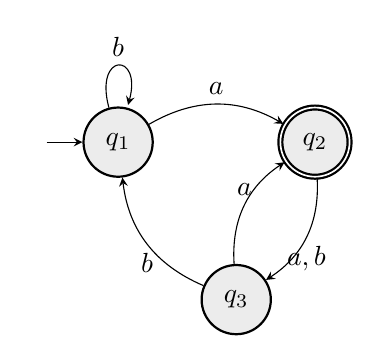
\begin{tikzpicture}
                  \node[state, initial] (q1) {$q_1$};
                  \node[state, accepting, right of=q1] (q2) {$q_2$};
                  \node[state] at (1.5, -2) (q3) {$q_3$};
                  \draw (q1) edge[loop above] node{$b$} (q1)
                  (q1) edge[bend left, above] node{$a$} (q2)
                  (q2) edge[bend left, below] node{$a,b$} (q3)
                  (q3) edge[bend left, above] node{$a$} (q2)
                  (q3) edge[bend left, below] node{$b$} (q1);
              \end{tikzpicture}
              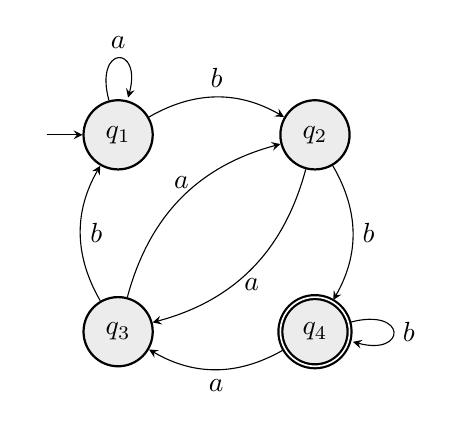
\begin{tikzpicture}
                  \node[state, initial] (q1) {$q_1$};
                  \node[state, right of=q1] (q2) {$q_2$};
                  \node[state, below of=q1] (q3) {$q_3$};
                  \node[state, accepting, below of=q2] (q4) {$q_4$};
                  \draw (q1) edge[loop above] node{$a$} (q1)
                  (q1) edge[bend left, above] node{$b$} (q2)
                  (q2) edge[bend left, below] node{$a$} (q3)
                  (q2) edge[bend left, right] node{$b$} (q4)
                  (q3) edge[bend left, above] node{$a$} (q2)
                  (q3) edge[bend left, right] node{$b$} (q1)
                  (q4) edge[bend left, below] node{$a$} (q3)
                  (q4) edge[loop right] node{$b$} (q4);
              \end{tikzpicture}
              \caption{$M_1$ and $M_2$}
          \end{figure}

          \begin{enumerate}
              \item What is the start state?

                    $M_1: q_1$

                    $M_2: q_1$

              \item What is the set of accept states?

                    $M_1: \{q_2\}$

                    $M_2: \{q_4\}$
              \item What sequence of states does the machine go through on input $aabb$?

                    $M_1: q_1 \rightarrow q_2 \rightarrow q_3 \rightarrow q_1 \rightarrow q_1$

                    $M_2: q_1 \rightarrow q_2 \rightarrow q_4 \rightarrow q_4 \rightarrow q_4$
              \item Does the machine accept the string $aabb$?

                    $M_1:$ No

                    $M_2:$ Yes
              \item Does the machine accept the string $\epsilon$?

                    $M_1:$ No

                    $M_2:$ No
          \end{enumerate}

    \item[1.2]

          Give the formal description of the machines $M_1$ and $M_2$ pictured in Exercise 1.1.

          $M_1 = (Q, \Sigma_1, \delta_1, q_1, \{q_2\})$

          $Q = \{q_1, q_2, q_3\}$

          $\Sigma_1 = \{a, b\}$

          $\delta_1 = \{((q_1, a), q_2), ((q_1, b), q_1), ((q_2, a), q_3), ((q_2, b), q_3), ((q_3, a), q_2), ((q_3, b), q_1)\}$\\

          $M_2 = (Q, \Sigma_2, \delta_2, q_1, \{q_4\})$

          $Q = \{q_1, q_2, q_3, q_4\}$

          $\Sigma_2 = \{a, b\}$

          $\delta_2 = \{((q_1, a), q_1), ((q_1, b), q_2), ((q_2, a), q_3), ((q_2, b), q_4),$\\
          .\,\,\,\qquad$((q_3, a), q_2), ((q_3, b), q_1), ((q_4, a), q_3), ((q_4, b), q_4)\}$

    \item[1.3]

          The formal description of a DFA $M$ is $\{q_1,q_2,q_3,q_4,q_5\},\{u,d\},\sigma,q_3,\{q_3\}$, where $\sigma$ is given by the following table. Give the state diagram of this machine.

          \begin{center}


              \begin{tabular}{ c | c c }
                        & $u$   & $d$   \\
                  \hline
                  $q_1$ & $q_1$ & $q_2$ \\
                  $q_2$ & $q_1$ & $q_3$ \\
                  $q_3$ & $q_2$ & $q_4$ \\
                  $q_4$ & $q_3$ & $q_5$ \\
                  $q_5$ & $q_4$ & $q_5$ \\
              \end{tabular}
          \end{center}

          \begin{figure}[H]
              \centering
              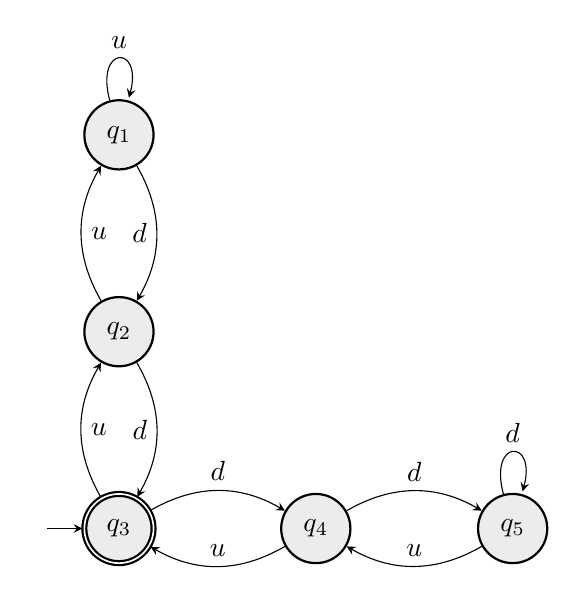
\begin{tikzpicture}
                  \node[state] (q1) {$q_1$};
                  \node[state, below of=q1] (q2) {$q_2$};
                  \node[state, accepting, initial, below of=q2] (q3) {$q_3$};
                  \node[state, right of=q3] (q4) {$q_4$};
                  \node[state, right of=q4] (q5) {$q_5$};
                  \draw (q1) edge[loop above] node{$u$} (q1)
                  (q1) edge[bend left, left] node{$d$} (q2)
                  (q2) edge[bend left, right] node{$u$} (q1)
                  (q2) edge[bend left, left] node{$d$} (q3)
                  (q3) edge[bend left, right] node{$u$} (q2)
                  (q3) edge[bend left, above] node{$d$} (q4)
                  (q4) edge[bend left, above] node{$u$} (q3)
                  (q4) edge[bend left, above] node{$d$} (q5)
                  (q5) edge[loop above] node{$d$} (q5)
                  (q5) edge[bend left, above] node{$u$} (q4);
              \end{tikzpicture}
          \end{figure}

    \item[1.4]
          Each of the following languages is the intersection of two simpler languages. In each part, construct DFAs for the simpler languages,then combine them using the construction discussed in footnote 3 (page 46) to give the state diagram of a DFA for the language given. In all parts, $\Sigma=\{a,b\}$.
          \begin{enumerate}
              \item $\{w|w~\text{has at least three }a\text{’s and at least two }b\text{’s}\}$

                    $DFA_1$ for at least three $a$'s:

                    \begin{figure}[H]
                        \centering
                        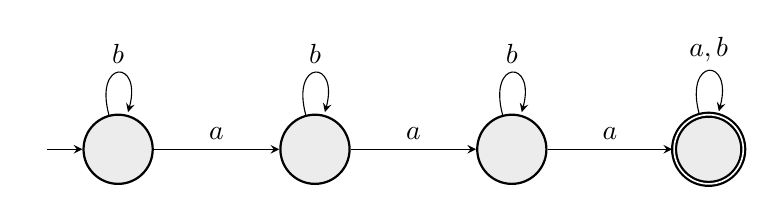
\begin{tikzpicture}
                            \node[state, initial] (q1) {};
                            \node[state, right of=q1] (q2) {};
                            \node[state, right of=q2] (q3) {};
                            \node[state, right of=q3, accepting] (q4) {};
                            \draw (q1) edge[loop above] node{$b$} (q1)
                            (q2) edge[loop above] node{$b$} (q2)
                            (q3) edge[loop above] node{$b$} (q3)
                            (q4) edge[loop above] node{$a,b$} (q4)
                            (q1) edge[left, above] node{$a$} (q2)
                            (q2) edge[left, above] node{$a$} (q3)
                            (q3) edge[left, above] node{$a$} (q4);
                        \end{tikzpicture}
                    \end{figure}

                    $DFA_2$ for at least two $b$'s:

                    \begin{figure}[H]
                        \centering
                        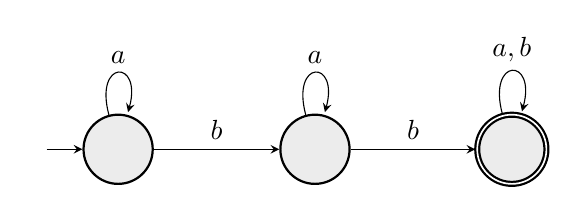
\begin{tikzpicture}
                            \node[state, initial] (q1) {};
                            \node[state, right of=q1] (q2) {};
                            \node[state, right of=q2, accepting] (q3) {};
                            \draw (q1) edge[loop above] node{$a$} (q1)
                            (q2) edge[loop above] node{$a$} (q2)
                            (q3) edge[loop above] node{$a,b$} (q3)
                            (q1) edge[left, above] node{$b$} (q2)
                            (q2) edge[left, above] node{$b$} (q3);
                        \end{tikzpicture}
                    \end{figure}

                    $DFA$ for at least three $a$'s and at least two $b$'s:

                    \begin{figure}[H]
                        \centering
                        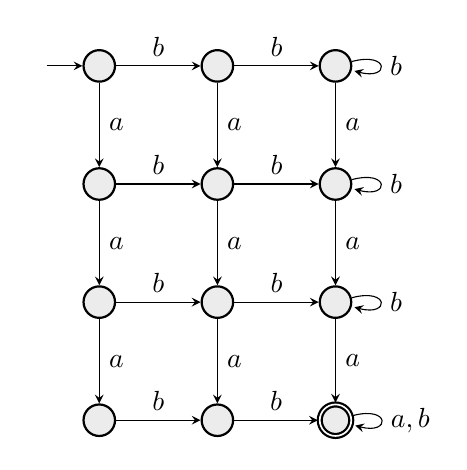
\begin{tikzpicture}[
                                styleSmall/.style={minimum size=4mm},
                                node distance=1.5cm,
                            ]
                            \node[state, initial, styleSmall] (q11) {};
                            \node[state, right of=q11, styleSmall] (q12) {};
                            \node[state, right of=q12, styleSmall] (q13) {};
                            \node[state, below of=q11, styleSmall] (q21) {};
                            \node[state, below of=q12, styleSmall] (q22) {};
                            \node[state, below of=q13, styleSmall] (q23) {};
                            \node[state, below of=q21, styleSmall] (q31) {};
                            \node[state, below of=q22, styleSmall] (q32) {};
                            \node[state, below of=q23, styleSmall] (q33) {};
                            \node[state, below of=q31, styleSmall] (q41) {};
                            \node[state, below of=q32, styleSmall] (q42) {};
                            \node[state, below of=q33, styleSmall, accepting] (q43) {};
                            \draw
                            (q13) edge[loop right] node{$b$} (q13)

                            (q11) edge[left, above] node{$b$} (q12)
                            (q12) edge[left, above] node{$b$} (q13)
                            (q23) edge[loop right] node{$b$} (q23)
                            (q21) edge[left, above] node{$b$} (q22)
                            (q22) edge[left, above] node{$b$} (q23)
                            (q33) edge[loop right] node{$b$} (q33)
                            (q31) edge[left, above] node{$b$} (q32)
                            (q32) edge[left, above] node{$b$} (q33)
                            (q43) edge[loop right] node{$a,b$} (q43)
                            (q41) edge[left, above] node{$b$} (q42)
                            (q42) edge[left, above] node{$b$} (q43)

                            (q11) edge[left, right] node{$a$} (q21)
                            (q12) edge[left, right] node{$a$} (q22)
                            (q13) edge[left, right] node{$a$} (q23)
                            (q21) edge[left, right] node{$a$} (q31)
                            (q22) edge[left, right] node{$a$} (q32)
                            (q23) edge[left, right] node{$a$} (q33)
                            (q31) edge[left, right] node{$a$} (q41)
                            (q32) edge[left, right] node{$a$} (q42)
                            (q33) edge[left, right] node{$a$} (q43);
                        \end{tikzpicture}
                    \end{figure}

              \item $\{w|w~\text{has exactly two }a\text{’s and at least two }b\text{’s}\}$

                    $DFA_1$ for exactly two $a$'s:

                    \begin{figure}[H]
                        \centering
                        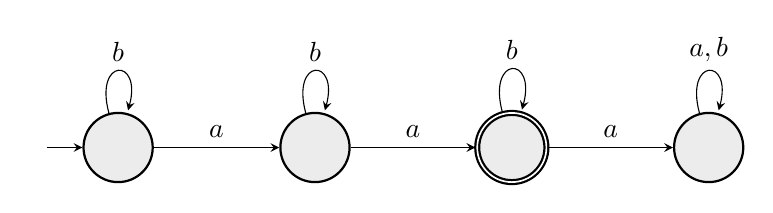
\begin{tikzpicture}
                            \node[state, initial] (q1) {};
                            \node[state, right of=q1] (q2) {};
                            \node[state, right of=q2, accepting] (q3) {};
                            \node[state, right of=q3] (q4) {};
                            \draw (q1) edge[loop above] node{$b$} (q1)
                            (q2) edge[loop above] node{$b$} (q2)
                            (q3) edge[loop above] node{$b$} (q3)
                            (q4) edge[loop above] node{$a,b$} (q4)
                            (q1) edge[left, above] node{$a$} (q2)
                            (q2) edge[left, above] node{$a$} (q3)
                            (q3) edge[left, above] node{$a$} (q4);
                        \end{tikzpicture}
                    \end{figure}

                    $DFA_2$ for at least two $b$'s:

                    \begin{figure}[H]
                        \centering
                        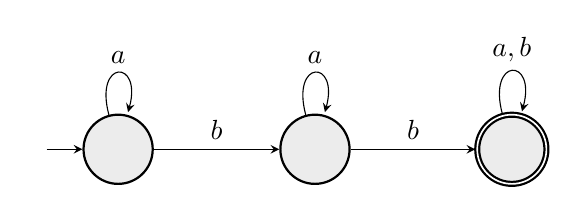
\begin{tikzpicture}
                            \node[state, initial] (q1) {};
                            \node[state, right of=q1] (q2) {};
                            \node[state, right of=q2, accepting] (q3) {};
                            \draw (q1) edge[loop above] node{$a$} (q1)
                            (q2) edge[loop above] node{$a$} (q2)
                            (q3) edge[loop above] node{$a,b$} (q3)
                            (q1) edge[left, above] node{$b$} (q2)
                            (q2) edge[left, above] node{$b$} (q3);
                        \end{tikzpicture}
                    \end{figure}

                    $DFA$ for exactly two $a$'s and at least two $b$'s:

                    \begin{figure}[H]
                        \centering
                        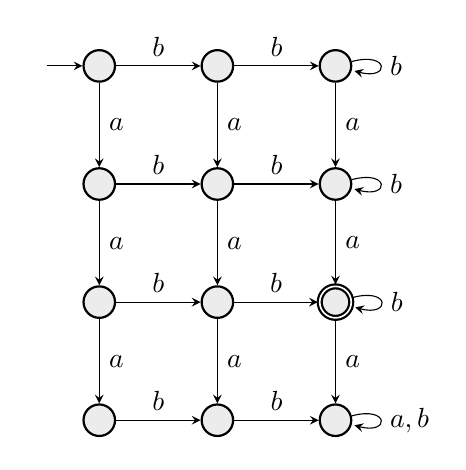
\begin{tikzpicture}[
                                styleSmall/.style={minimum size=4mm},
                                node distance=1.5cm,
                            ]
                            \node[state, initial, styleSmall] (q11) {};
                            \node[state, right of=q11, styleSmall] (q12) {};
                            \node[state, right of=q12, styleSmall] (q13) {};
                            \node[state, below of=q11, styleSmall] (q21) {};
                            \node[state, below of=q12, styleSmall] (q22) {};
                            \node[state, below of=q13, styleSmall] (q23) {};
                            \node[state, below of=q21, styleSmall] (q31) {};
                            \node[state, below of=q22, styleSmall] (q32) {};
                            \node[state, below of=q23, styleSmall, accepting] (q33) {};
                            \node[state, below of=q31, styleSmall] (q41) {};
                            \node[state, below of=q32, styleSmall] (q42) {};
                            \node[state, below of=q33, styleSmall] (q43) {};
                            \draw
                            (q13) edge[loop right] node{$b$} (q13)
                            (q11) edge[left, above] node{$b$} (q12)
                            (q12) edge[left, above] node{$b$} (q13)
                            (q23) edge[loop right] node{$b$} (q23)
                            (q21) edge[left, above] node{$b$} (q22)
                            (q22) edge[left, above] node{$b$} (q23)
                            (q33) edge[loop right] node{$b$} (q33)
                            (q31) edge[left, above] node{$b$} (q32)
                            (q32) edge[left, above] node{$b$} (q33)
                            (q43) edge[loop right] node{$a,b$} (q43)
                            (q41) edge[left, above] node{$b$} (q42)
                            (q42) edge[left, above] node{$b$} (q43)

                            (q11) edge[left, right] node{$a$} (q21)
                            (q12) edge[left, right] node{$a$} (q22)
                            (q13) edge[left, right] node{$a$} (q23)
                            (q21) edge[left, right] node{$a$} (q31)
                            (q22) edge[left, right] node{$a$} (q32)
                            (q23) edge[left, right] node{$a$} (q33)
                            (q31) edge[left, right] node{$a$} (q41)
                            (q32) edge[left, right] node{$a$} (q42)
                            (q33) edge[left, right] node{$a$} (q43);
                        \end{tikzpicture}
                    \end{figure}

              \item $\{w|w~\text{has an even number of }a\text{’s and one or two }b\text{’s}\}$

                    $DFA_1$ for an even number of $a$'s:

                    \begin{figure}[H]
                        \centering
                        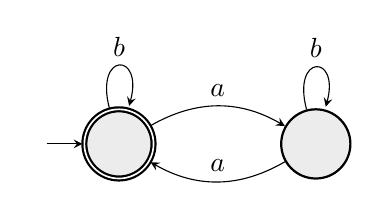
\begin{tikzpicture}
                            \node[state, initial, accepting] (q1) {};
                            \node[state, right of=q1] (q2) {};
                            \draw (q1) edge[loop above] node{$b$} (q1)
                            (q2) edge[loop above] node{$b$} (q2)
                            (q1) edge[bend left, above] node{$a$} (q2)
                            (q2) edge[bend left, above] node{$a$} (q1);
                        \end{tikzpicture}
                    \end{figure}

                    $DFA_2$ for one or two $b$'s:

                    \begin{figure}[H]
                        \centering
                        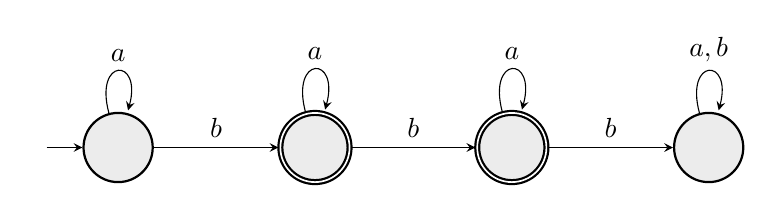
\begin{tikzpicture}
                            \node[state, initial] (q1) {};
                            \node[state, right of=q1, accepting] (q2) {};
                            \node[state, right of=q2, accepting] (q3) {};
                            \node[state, right of=q3] (q4) {};
                            \draw (q1) edge[loop above] node{$a$} (q1)
                            (q2) edge[loop above] node{$a$} (q2)
                            (q3) edge[loop above] node{$a$} (q3)
                            (q4) edge[loop above] node{$a,b$} (q4)
                            (q1) edge[left, above] node{$b$} (q2)
                            (q2) edge[left, above] node{$b$} (q3)
                            (q3) edge[left, above] node{$b$} (q4);
                        \end{tikzpicture}
                    \end{figure}

                    $DFA$ for an even number of $a$'s and one or two $b$'s:

                    \begin{figure}[H]
                        \centering
                        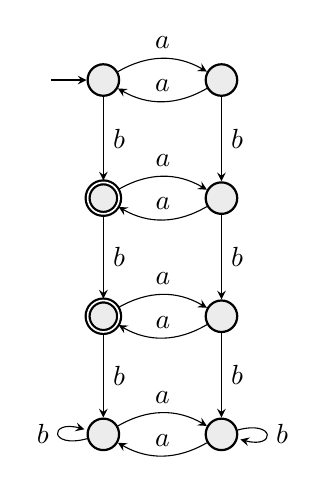
\begin{tikzpicture}[
                                styleSmall/.style={minimum size=4mm},
                                node distance=1.5cm,
                            ]
                            \node[state, initial, styleSmall] (q11) {};
                            \node[state, right of=q11, styleSmall] (q12) {};
                            \node[state, below of=q11, styleSmall, accepting] (q21) {};
                            \node[state, below of=q12, styleSmall] (q22) {};
                            \node[state, below of=q21, styleSmall, accepting] (q31) {};
                            \node[state, below of=q22, styleSmall] (q32) {};
                            \node[state, below of=q31, styleSmall] (q41) {};
                            \node[state, below of=q32, styleSmall] (q42) {};
                            \draw
                            (q11) edge[bend left, above] node{$a$} (q12)
                            (q12) edge[bend left, above] node{$a$} (q11)
                            (q21) edge[bend left, above] node{$a$} (q22)
                            (q22) edge[bend left, above] node{$a$} (q21)
                            (q31) edge[bend left, above] node{$a$} (q32)
                            (q32) edge[bend left, above] node{$a$} (q31)
                            (q41) edge[bend left, above] node{$a$} (q42)
                            (q42) edge[bend left, above] node{$a$} (q41)

                            (q41) edge[loop left] node{$b$} (q41)
                            (q42) edge[loop right] node{$b$} (q42)

                            (q11) edge[left, right] node{$b$} (q21)
                            (q12) edge[left, right] node{$b$} (q22)
                            (q21) edge[left, right] node{$b$} (q31)
                            (q22) edge[left, right] node{$b$} (q32)
                            (q31) edge[left, right] node{$b$} (q41)
                            (q32) edge[left, right] node{$b$} (q42);
                        \end{tikzpicture}
                    \end{figure}


              \item $\{w|w~\text{has an even number of }a\text{’s and each }a\text{ is followed by at least one }b\}$

                    $DFA_1$ for an even number of $a$'s:

                    \begin{figure}[H]
                        \centering
                        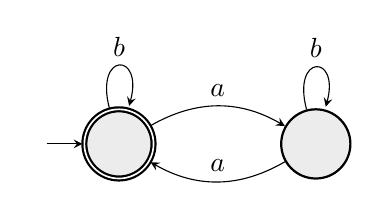
\begin{tikzpicture}
                            \node[state, initial, accepting] (q1) {};
                            \node[state, right of=q1] (q2) {};
                            \draw (q1) edge[loop above] node{$b$} (q1)
                            (q2) edge[loop above] node{$b$} (q2)
                            (q1) edge[bend left, above] node{$a$} (q2)
                            (q2) edge[bend left, above] node{$a$} (q1);
                        \end{tikzpicture}
                    \end{figure}

                    $DFA_2$ for each $a$ is followed by at least one $b$:

                    \begin{figure}[H]
                        \centering
                        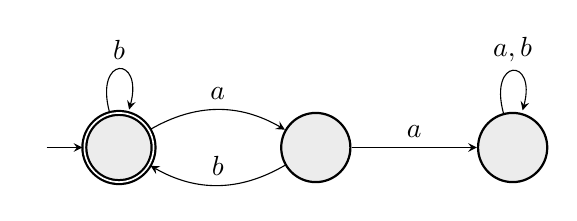
\begin{tikzpicture}
                            \node[state, initial, accepting] (q1) {};
                            \node[state, right of=q1] (q2) {};
                            \node[state, right of=q2] (q3) {};
                            \draw (q1) edge[loop above] node{$b$} (q1)
                            (q3) edge[loop above] node{$a,b$} (q3)
                            (q1) edge[bend left, above] node{$a$} (q2)
                            (q2) edge[bend left, above] node{$b$} (q1)
                            (q2) edge[left, above] node{$a$} (q3);
                        \end{tikzpicture}
                    \end{figure}

              \item $\{w|w~\text{starts with an }a\text{ and has at most one }b\}$

                    $DFA_1$ for starts with an $a$:

                    \begin{figure}[H]
                        \centering
                        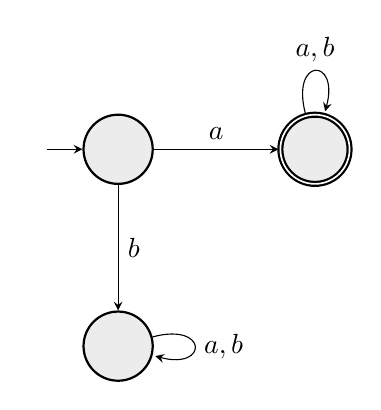
\begin{tikzpicture}
                            \node[state, initial] (q1) {};
                            \node[state, right of=q1, accepting] (q2) {};
                            \node[state, below of=q1 ] (q3) {};
                            \draw
                            (q3) edge[loop right] node{$a,b$} (q3)
                            (q2) edge[loop above] node{$a,b$} (q2)
                            (q1) edge[above] node{$a$} (q2)
                            (q1) edge[right] node{$b$} (q3);
                        \end{tikzpicture}
                    \end{figure}

                    $DFA_2$ for has at most one $b$:

                    \begin{figure}[H]
                        \centering
                        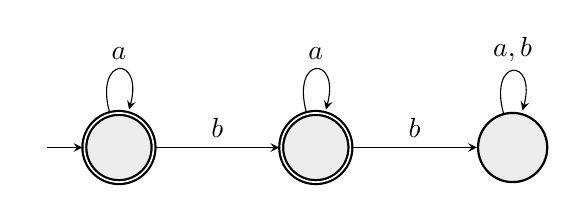
\begin{tikzpicture}
                            \node[state, initial, accepting] (q1) {};
                            \node[state, right of=q1, accepting] (q2) {};
                            \node[state, right of=q2] (q3) {};
                            \draw (q1) edge[loop above] node{$a$} (q1)
                            (q2) edge[loop above] node{$a$} (q2)
                            (q3) edge[loop above] node{$a,b$} (q3)
                            (q1) edge[left, above] node{$b$} (q2)
                            (q2) edge[left, above] node{$b$} (q3);
                        \end{tikzpicture}
                    \end{figure}

              \item $\{w|w~\text{has an odd number of }a\text{’s and ends with a }b\}$

                    $DFA_1$ for an odd number of $a$'s:

                    \begin{figure}[H]
                        \centering
                        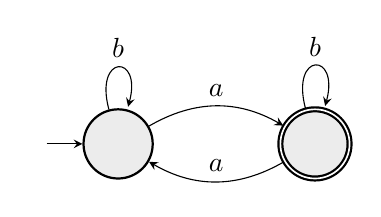
\begin{tikzpicture}
                            \node[state, initial] (q1) {};
                            \node[state, right of=q1, accepting] (q2) {};
                            \draw (q1) edge[loop above] node{$b$} (q1)
                            (q2) edge[loop above] node{$b$} (q2)
                            (q1) edge[bend left, above] node{$a$} (q2)
                            (q2) edge[bend left, above] node{$a$} (q1);
                        \end{tikzpicture}
                    \end{figure}

                    $DFA_2$ for ends with a $b$:

                    \begin{figure}[H]
                        \centering
                        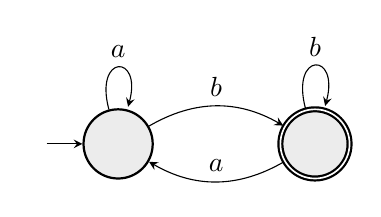
\begin{tikzpicture}
                            \node[state, initial] (q1) {};
                            \node[state, right of=q1, accepting] (q2) {};
                            \draw (q1) edge[loop above] node{$a$} (q1)
                            (q2) edge[loop above] node{$b$} (q2)
                            (q1) edge[bend left, above] node{$b$} (q2)
                            (q2) edge[bend left, above] node{$a$} (q1);
                        \end{tikzpicture}
                    \end{figure}

              \item $\{w|w~\text{has even length and an odd number of }a\text{’s}\}$

                    $DFA_1$ for even length:

                    \begin{figure}[H]
                        \centering
                        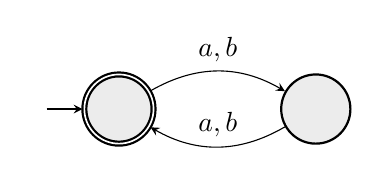
\begin{tikzpicture}
                            \node[state, initial, accepting] (q1) {};
                            \node[state, right of=q1] (q2) {};
                            \draw
                            (q1) edge[bend left, above] node{$a,b$} (q2)
                            (q2) edge[bend left, above] node{$a,b$} (q1);
                        \end{tikzpicture}
                    \end{figure}

                    $DFA_2$ for an odd number of $a$'s:

                    \begin{figure}[H]
                        \centering
                        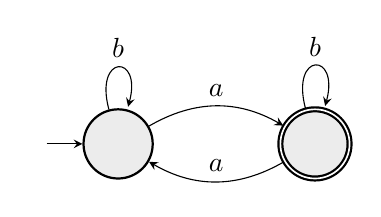
\begin{tikzpicture}
                            \node[state, initial] (q1) {};
                            \node[state, right of=q1, accepting] (q2) {};
                            \draw (q1) edge[loop above] node{$b$} (q1)
                            (q2) edge[loop above] node{$b$} (q2)
                            (q1) edge[bend left, above] node{$a$} (q2)
                            (q2) edge[bend left, above] node{$a$} (q1);
                        \end{tikzpicture}
                    \end{figure}

          \end{enumerate}

    \item[1.5]
          Each of the following languages is the complement of a simpler language. In each part, construct a DFA for the simpler language, then use it to give the state diagram of a DFA for the language given. In all parts, $\Sigma=\{a,b\}$.
          \begin{enumerate}
              \item $A = \{w|w~\text{does not contain the substring }ab\}$

                    $\overline{A} = \{w|w~\text{contains the substring }ab\}$
                    \begin{figure}[H]
                        \centering
                        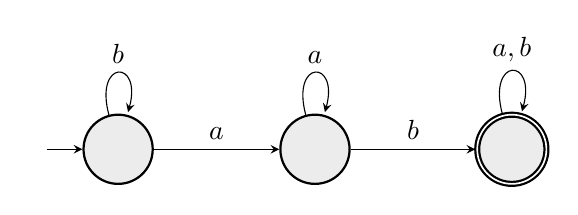
\begin{tikzpicture}
                            \node[state, initial] (q1) {};
                            \node[state, right of=q1] (q2) {};
                            \node[state, accepting, right of=q2] (q3) {};
                            \draw (q1) edge[left, above] node{$a$} (q2)
                            (q1) edge[loop above] node{$b$} (q1)
                            (q2) edge[left, above] node{$b$} (q3)
                            (q2) edge[loop above] node{$a$} (q2)
                            (q3) edge[loop above] node{$a,b$} (q3);
                        \end{tikzpicture}
                        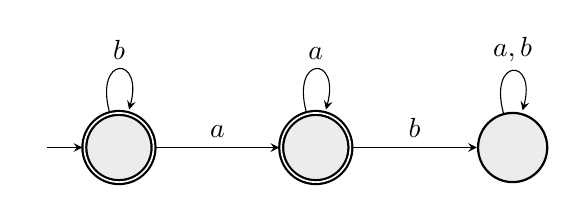
\begin{tikzpicture}
                            \node[state, accepting, initial] (q1) {};
                            \node[state, accepting, right of=q1] (q2) {};
                            \node[state, right of=q2] (q3) {};
                            \draw (q1) edge[left, above] node{$a$} (q2)
                            (q1) edge[loop above] node{$b$} (q1)
                            (q2) edge[left, above] node{$b$} (q3)
                            (q2) edge[loop above] node{$a$} (q2)
                            (q3) edge[loop above] node{$a,b$} (q3);
                        \end{tikzpicture}
                        \caption{$\overline{A}$ and $A$}
                    \end{figure}
              \item $B = \{w|w~\text{does notcontain the substring }baba\}$

                    $\overline{B} = \{w|w~\text{contains the substring }baba\}$
                    \begin{figure}[H]
                        \centering
                        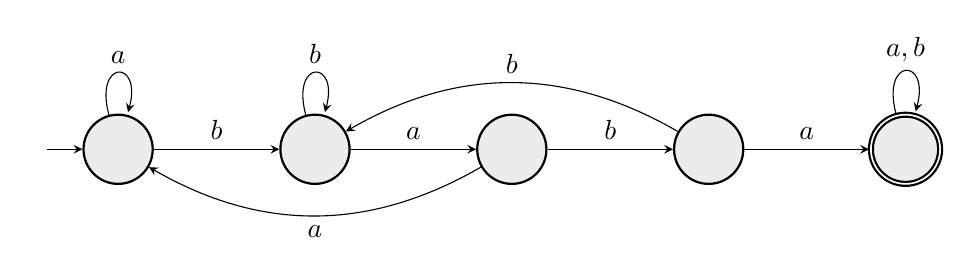
\begin{tikzpicture}
                            \node[state, initial] (q1) {};
                            \node[state, right of=q1] (q2) {};
                            \node[state, right of=q2] (q3) {};
                            \node[state, right of=q3] (q4) {};
                            \node[state, accepting, right of=q4] (q5) {};
                            \draw (q1) edge[left, above] node{$b$} (q2)
                            (q1) edge[loop above] node{$a$} (q1)
                            (q2) edge[left, above] node{$a$} (q3)
                            (q2) edge[loop above] node{$b$} (q2)
                            (q3) edge[left, above] node{$b$} (q4)
                            (q3) edge[bend left, below] node{$a$} (q1)
                            (q4) edge[bend right, above] node{$b$} (q2)
                            (q4) edge[left, above] node{$a$} (q5)
                            (q5) edge[loop above] node{$a,b$} (q5);
                        \end{tikzpicture}
                        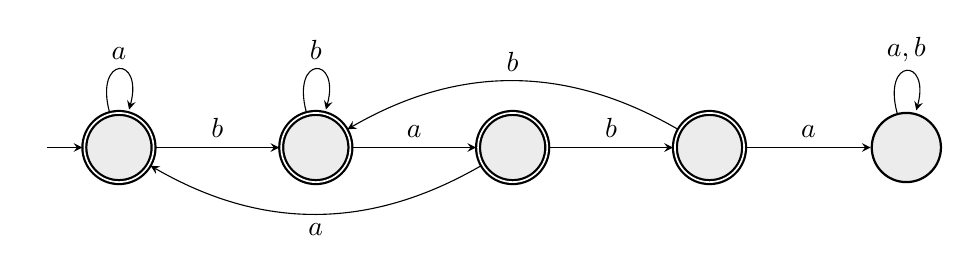
\begin{tikzpicture}
                            \node[state, accepting, initial] (q1) {};
                            \node[state, accepting, right of=q1] (q2) {};
                            \node[state, accepting, right of=q2] (q3) {};
                            \node[state, accepting, right of=q3] (q4) {};
                            \node[state, right of=q4] (q5) {};
                            \draw (q1) edge[left, above] node{$b$} (q2)
                            (q1) edge[loop above] node{$a$} (q1)
                            (q2) edge[left, above] node{$a$} (q3)
                            (q2) edge[loop above] node{$b$} (q2)
                            (q3) edge[left, above] node{$b$} (q4)
                            (q3) edge[bend left, below] node{$a$} (q1)
                            (q4) edge[bend right, above] node{$b$} (q2)
                            (q4) edge[left, above] node{$a$} (q5)
                            (q5) edge[loop above] node{$a,b$} (q5);
                        \end{tikzpicture}
                        \caption{$\overline{B}$ and $B$}
                    \end{figure}

              \item $C =\{w|w~\text{contains neither the substrings }ab\text{ nor }ba\}$

                    $\overline{C} = \{w|w~\text{contains the substring }ab\text{ or }ba\}$
                    \begin{figure}[H]
                        \centering
                        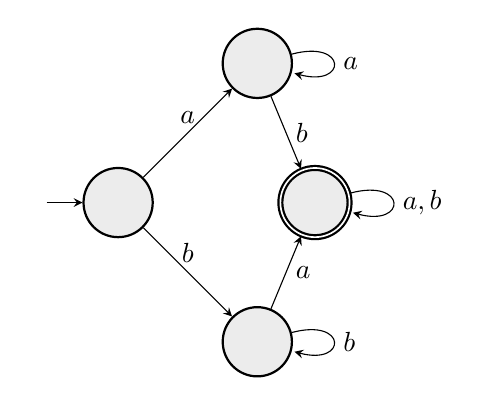
\begin{tikzpicture}
                            \node[state, initial] (q1) {};
                            \node[state, above right of=q1] (q2) {};
                            \node[state, below right of=q1] (q3) {};
                            \node[state, accepting, right of=q1] (q4) {};
                            \draw (q1) edge[left, above] node{$a$} (q2)
                            (q1) edge[left, above] node{$b$} (q3)
                            (q2) edge[right] node{$b$} (q4)
                            (q2) edge[loop right] node{$a$} (q2)
                            (q3) edge[right] node{$a$} (q4)
                            (q3) edge[loop right] node{$b$} (q3)
                            (q4) edge[loop right] node{$a,b$} (q4);
                        \end{tikzpicture}
                        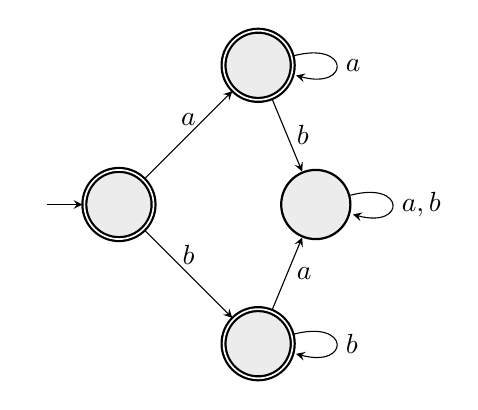
\begin{tikzpicture}
                            \node[state, accepting, initial] (q1) {};
                            \node[state, accepting, above right of=q1] (q2) {};
                            \node[state, accepting, below right of=q1] (q3) {};
                            \node[state, right of=q1] (q4) {};
                            \draw (q1) edge[left, above] node{$a$} (q2)
                            (q1) edge[left, above] node{$b$} (q3)
                            (q2) edge[right] node{$b$} (q4)
                            (q2) edge[loop right] node{$a$} (q2)
                            (q3) edge[right] node{$a$} (q4)
                            (q3) edge[loop right] node{$b$} (q3)
                            (q4) edge[loop right] node{$a,b$} (q4);
                        \end{tikzpicture}
                        \caption{$\overline{C}$ and $C$}
                    \end{figure}
              \item $D = \{w|w~\text{is any string not in }a^{\ast}b^{\ast}\}$

                    $\overline{D} = \{w|w~\text{is any string in }a^{\ast}b^{\ast}\}$
                    \begin{figure}[H]
                        \centering
                        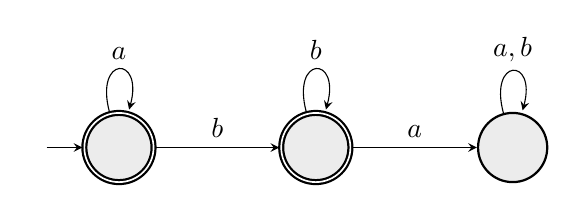
\begin{tikzpicture}
                            \node[state, accepting, initial] (q1) {};
                            \node[state, accepting, right of=q1] (q2) {};
                            \node[state, right of=q2] (q3) {};
                            \draw (q1) edge[loop above] node{$a$} (q1)
                            (q1) edge[above] node{$b$} (q2)
                            (q2) edge[loop above] node{$b$} (q2)
                            (q2) edge[above] node{$a$} (q3)
                            (q3) edge[loop above] node{$a,b$} (q3);
                        \end{tikzpicture}
                        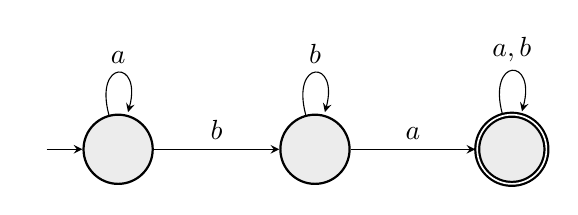
\begin{tikzpicture}
                            \node[state, initial] (q1) {};
                            \node[state, right of=q1] (q2) {};
                            \node[state, accepting, right of=q2] (q3) {};
                            \draw (q1) edge[loop above] node{$a$} (q1)
                            (q1) edge[above] node{$b$} (q2)
                            (q2) edge[loop above] node{$b$} (q2)
                            (q2) edge[above] node{$a$} (q3)
                            (q3) edge[loop above] node{$a,b$} (q3);
                        \end{tikzpicture}
                        \caption{$\overline{D}$ and $D$}
                    \end{figure}
              \item $E = \{w|w~\text{is any string not in }(ab^+)^{\ast}\}$

                    $\overline{E} = \{w|w~\text{is any string in }(ab^+)^{\ast}\}$

                    \begin{itemize}
                        \item assuming $ab^+$ means $a$ followed by one or more $b$.
                              \begin{figure}[H]
                                  \centering
                                  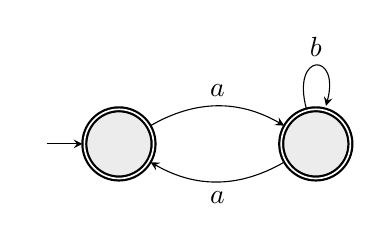
\begin{tikzpicture}
                                      \node[state, accepting, initial] (q1) {};
                                      \node[state, accepting, right of=q1] (q2) {};
                                      \draw (q1) edge[bend left, above] node{$a$} (q2)
                                      (q2) edge[bend left, below] node{$a$} (q1)
                                      (q2) edge[loop above] node{$b$} (q2);
                                  \end{tikzpicture}
                                  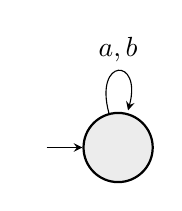
\begin{tikzpicture}
                                      \node[state, initial] (q1) {};
                                      \draw (q1) edge[loop above] node{$a,b$} (q1);
                                  \end{tikzpicture}
                                  \caption{$\overline{E}$ and $E$}
                              \end{figure}
                        \item assuming $ab^+$ means $ab$ one or more times.
                              \begin{figure}[H]
                                  \centering
                                  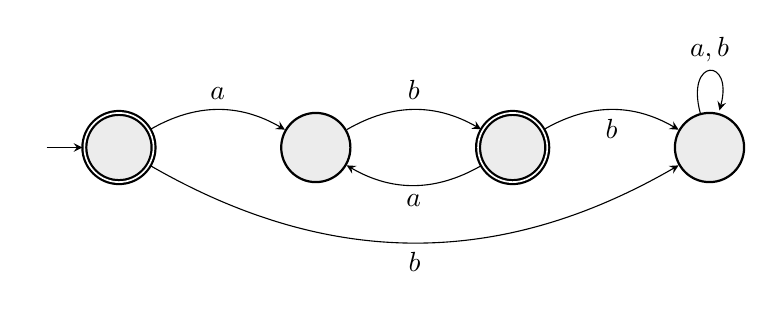
\begin{tikzpicture}
                                      \node[state, accepting, initial] (q1) {};
                                      \node[state, right of=q1] (q2) {};
                                      \node[state, accepting, right of=q2] (q3) {};
                                      \node[state, right of=q3] (q4) {};
                                      \draw (q1) edge[bend left, above] node{$a$} (q2)
                                      (q2) edge[bend left, above] node{$b$} (q3)
                                      (q3) edge[bend left, below] node{$a$} (q2)
                                      (q3) edge[bend left, below] node{$b$} (q4)
                                      (q1) edge[bend right, below] node{$b$} (q4)
                                      (q4) edge[loop above] node{$a,b$} (q4);
                                  \end{tikzpicture}
                                  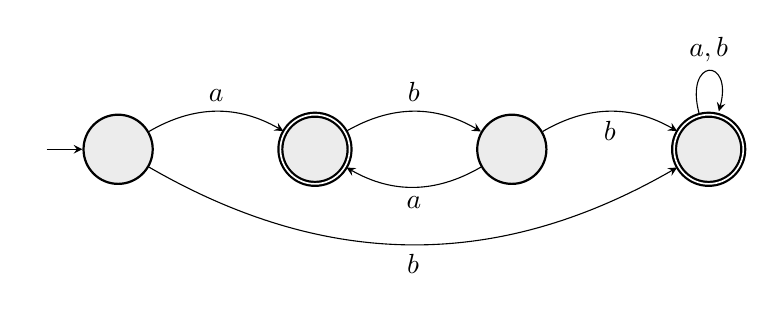
\begin{tikzpicture}
                                      \node[state, initial] (q1) {};
                                      \node[state, accepting, right of=q1] (q2) {};
                                      \node[state, right of=q2] (q3) {};
                                      \node[state, accepting, right of=q3] (q4) {};
                                      \draw (q1) edge[bend left, above] node{$a$} (q2)
                                      (q2) edge[bend left, above] node{$b$} (q3)
                                      (q3) edge[bend left, below] node{$a$} (q2)
                                      (q3) edge[bend left, below] node{$b$} (q4)
                                      (q1) edge[bend right, below] node{$b$} (q4)
                                      (q4) edge[loop above] node{$a,b$} (q4);
                                  \end{tikzpicture}
                                  \caption{$\overline{E}$ and $E$}
                              \end{figure}
                    \end{itemize}
              \item $F = \{w|w~\text{is any string not in }a^{\ast} \cup b^{\ast}\}$

                    $\overline{F} = \{w|w~\text{is any string in }a^{\ast} \cup b^{\ast}\}$
                    \begin{figure}[H]
                        \centering
                        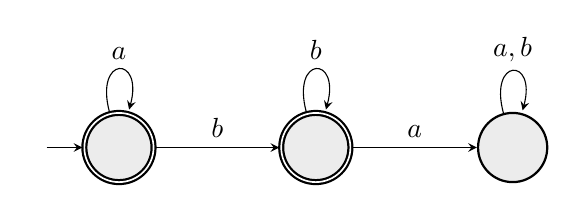
\begin{tikzpicture}
                            \node[state, accepting, initial] (q1) {};
                            \node[state, accepting, right of=q1] (q2) {};
                            \node[state, right of=q2] (q3) {};
                            \draw (q1) edge[loop above] node{$a$} (q1)
                            (q1) edge[above] node{$b$} (q2)
                            (q2) edge[loop above] node{$b$} (q2)
                            (q2) edge[above] node{$a$} (q3)
                            (q3) edge[loop above] node{$a,b$} (q3);
                        \end{tikzpicture}
                        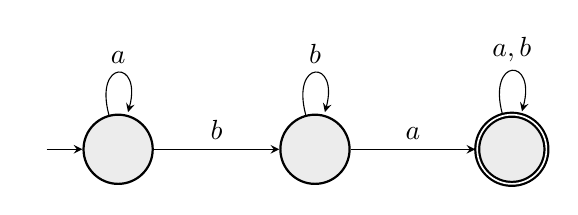
\begin{tikzpicture}
                            \node[state, initial] (q1) {};
                            \node[state, right of=q1] (q2) {};
                            \node[state, accepting, right of=q2] (q3) {};
                            \draw (q1) edge[loop above] node{$a$} (q1)
                            (q1) edge[above] node{$b$} (q2)
                            (q2) edge[loop above] node{$b$} (q2)
                            (q2) edge[above] node{$a$} (q3)
                            (q3) edge[loop above] node{$a,b$} (q3);
                        \end{tikzpicture}
                        \caption{$\overline{F}$ and $F$}
                    \end{figure}
              \item $G= \{w|w~\text{is any string that doesn’t contain exactly two }a\text{’s}\}$

                    $\overline{G} = \{w|w~\text{is any string that contains exactly two }a\text{’s}\}$
                    \begin{figure}[H]
                        \centering
                        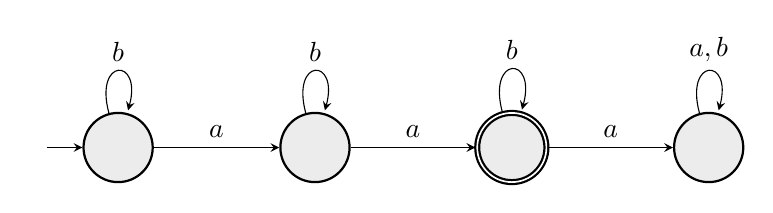
\begin{tikzpicture}
                            \node[state, initial] (q1) {};
                            \node[state, right of=q1] (q2) {};
                            \node[state, accepting, right of=q2] (q3) {};
                            \node[state, right of=q3] (q4) {};
                            \draw (q1) edge[loop above] node{$b$} (q1)
                            (q1) edge[above] node{$a$} (q2)
                            (q2) edge[loop above] node{$b$} (q2)
                            (q2) edge[above] node{$a$} (q3)
                            (q3) edge[loop above] node{$b$} (q3)
                            (q3) edge[above] node{$a$} (q4)
                            (q4) edge[loop above] node{$a,b$} (q4);
                        \end{tikzpicture}
                        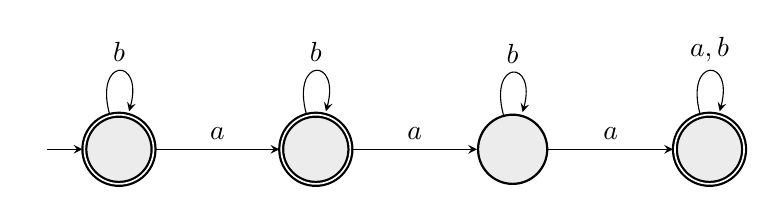
\begin{tikzpicture}
                            \node[state, accepting, initial] (q1) {};
                            \node[state, accepting, right of=q1] (q2) {};
                            \node[state, right of=q2] (q3) {};
                            \node[state, accepting, right of=q3] (q4) {};
                            \draw (q1) edge[loop above] node{$b$} (q1)
                            (q1) edge[above] node{$a$} (q2)
                            (q2) edge[loop above] node{$b$} (q2)
                            (q2) edge[above] node{$a$} (q3)
                            (q3) edge[loop above] node{$b$} (q3)
                            (q3) edge[above] node{$a$} (q4)
                            (q4) edge[loop above] node{$a,b$} (q4);
                        \end{tikzpicture}
                        \caption{$\overline{G}$ and $G$}
                    \end{figure}
              \item $H=\{w|w~\text{is any string except }a\text{ and }b\}$

                    $\overline{H} = \{w|w~\text{is string }a\text{ or }b\}$
                    \begin{figure}[H]
                        \centering
                        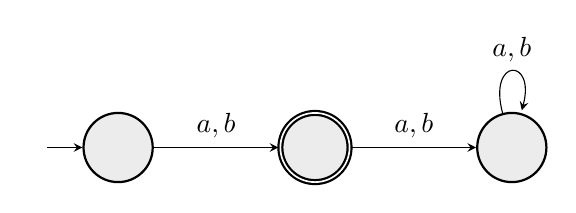
\begin{tikzpicture}
                            \node[state, initial] (q1) {};
                            \node[state, accepting, right of=q1] (q2) {};
                            \node[state, right of=q2] (q3) {};
                            \draw
                            (q1) edge[above] node{$a,b$} (q2)
                            (q2) edge[above] node{$a,b$} (q3)
                            (q3) edge[loop above] node{$a,b$} (q3);
                        \end{tikzpicture}
                        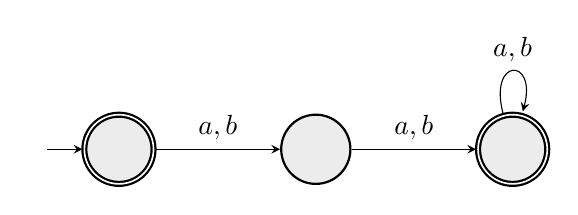
\begin{tikzpicture}
                            \node[state, accepting, initial] (q1) {};
                            \node[state, right of=q1] (q2) {};
                            \node[state, accepting, right of=q2] (q3) {};
                            \draw
                            (q1) edge[above] node{$a,b$} (q2)
                            (q2) edge[above] node{$a,b$} (q3)
                            (q3) edge[loop above] node{$a,b$} (q3);
                        \end{tikzpicture}
                        \caption{$\overline{H}$ and $H$}
                    \end{figure}
          \end{enumerate}

    \item[1.6]
          Give state diagrams of DFAs recognizing the following languages. In all parts,the alphabet is $\{0,1\}$.
          \begin{enumerate}
              \item $\{w|w~ \text{begins with a }1\text{ and ends with a }0\}$
                    \begin{figure}[H]
                        \centering
                        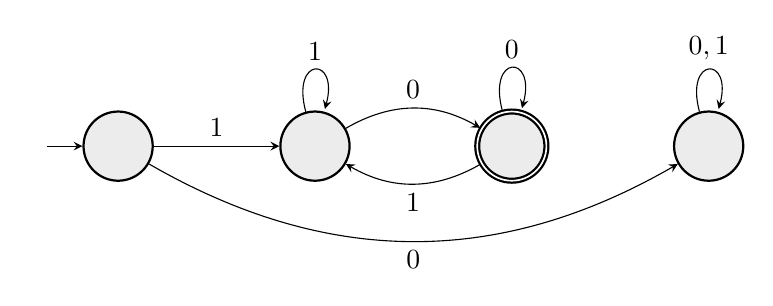
\begin{tikzpicture}
                            \node[state, initial] (q1) {};
                            \node[state, right of=q1] (q2) {};
                            \node[state, accepting, right of=q2] (q3) {};
                            \node[state, right of=q3] (q4) {};
                            \draw
                            (q1) edge[above] node{$1$} (q2)
                            (q2) edge[loop above] node{$1$} (q2)
                            (q2) edge[bend left, above] node{$0$} (q3)
                            (q3) edge[loop above] node{$0$} (q3)
                            (q3) edge[bend left, below] node{$1$} (q2)
                            (q1) edge[bend right, below] node{$0$} (q4)
                            (q4) edge[loop above] node{$0,1$} (q4);
                        \end{tikzpicture}
                    \end{figure}
              \item $\{w|w~ \text{contains at least three }1\text{'s}\}$
                    \begin{figure}[H]
                        \centering
                        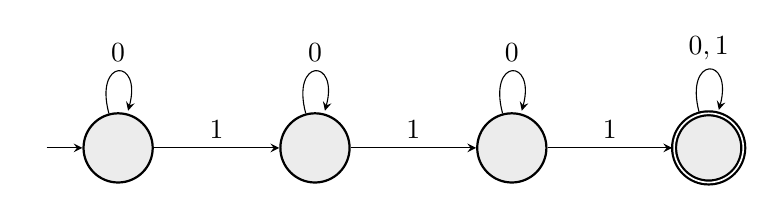
\begin{tikzpicture}
                            \node[state, initial] (q1) {};
                            \node[state, right of=q1] (q2) {};
                            \node[state, right of=q2] (q3) {};
                            \node[state, accepting, right of=q3] (q4) {};
                            \draw
                            (q1) edge[loop above] node{$0$} (q1)
                            (q1) edge[above] node{$1$} (q2)
                            (q2) edge[loop above] node{$0$} (q2)
                            (q2) edge[above] node{$1$} (q3)
                            (q3) edge[loop above] node{$0$} (q3)
                            (q3) edge[above] node{$1$} (q4)
                            (q4) edge[loop above] node{$0,1$} (q4);
                        \end{tikzpicture}
                    \end{figure}
              \item $\{w|w~ \text{contains the substring } 0101~ \text{(i.e., }w = x0101y\text{ for some }x\text{ and }y)\}$
                    \begin{figure}[H]
                        \centering
                        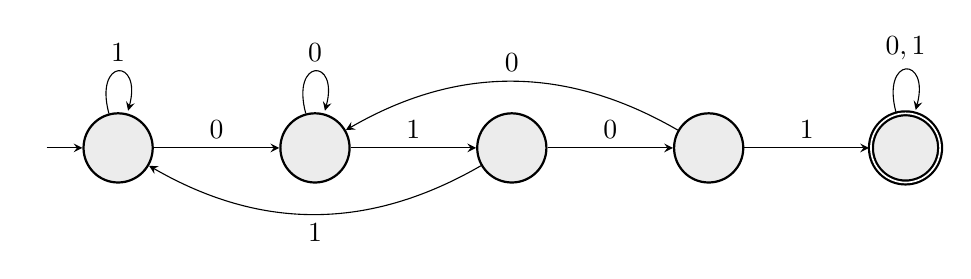
\begin{tikzpicture}
                            \node[state, initial] (q1) {};
                            \node[state, right of=q1] (q2) {};
                            \node[state, right of=q2] (q3) {};
                            \node[state, right of=q3] (q4) {};
                            \node[state, accepting, right of=q4] (q5) {};
                            \draw
                            (q1) edge[loop above] node{$1$} (q1)
                            (q1) edge[above] node{$0$} (q2)
                            (q2) edge[loop above] node{$0$} (q2)
                            (q2) edge[above] node{$1$} (q3)
                            (q3) edge[above] node{$0$} (q4)
                            (q4) edge[above] node{$1$} (q5)
                            (q5) edge[loop above] node{$0,1$} (q5)
                            (q3) edge[bend left, below] node{$1$} (q1)
                            (q4) edge[bend right, above] node{$0$} (q2);
                        \end{tikzpicture}
                    \end{figure}
              \item $\{w|w~ \text{has length at least }3\text{ and its third symbol is a }0\}$
                    \begin{figure}[H]
                        \centering
                        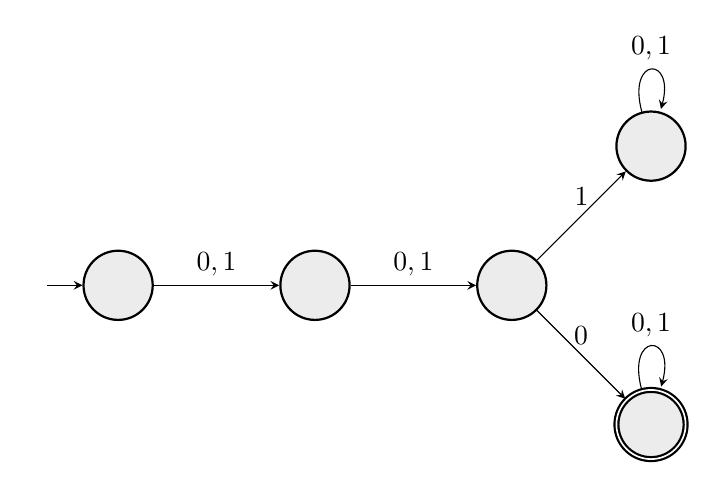
\begin{tikzpicture}
                            \node[state, initial] (q1) {};
                            \node[state, right of=q1] (q2) {};
                            \node[state, right of=q2] (q3) {};
                            \node[state, accepting, below right of=q3] (q4) {};
                            \node[state, above right of=q3] (q5) {};
                            \draw
                            (q1) edge[above] node{$0,1$} (q2)
                            (q2) edge[above] node{$0,1$} (q3)
                            (q3) edge[above] node{$0$} (q4)
                            (q3) edge[above] node{$1$} (q5)
                            (q4) edge[loop above] node{$0,1$} (q4)
                            (q5) edge[loop above] node{$0,1$} (q5);
                        \end{tikzpicture}
                    \end{figure}

              \item $\{w|w~ \text{starts with }0\text{ and has odd length, or starts with }1\text{ and has even length}\}$
                    \begin{figure}[H]
                        \centering
                        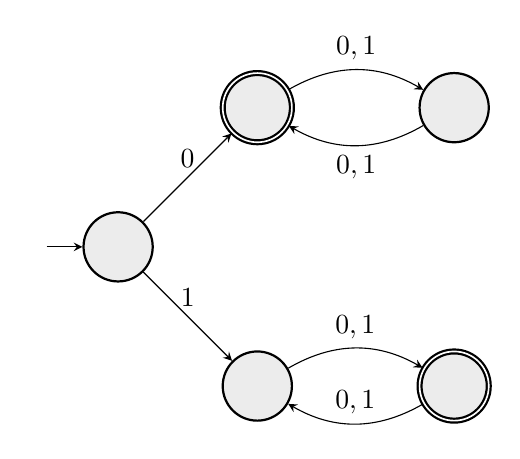
\begin{tikzpicture}
                            \node[state, initial] (q1) {};
                            \node[state, accepting, above right of=q1] (q2) {};
                            \node[state, below right of=q1] (q3) {};
                            \node[state, right of=q2] (q4) {};
                            \node[state, accepting, right of=q3] (q5) {};
                            \draw
                            (q1) edge[above] node{$0$} (q2)
                            (q1) edge[above] node{$1$} (q3)
                            (q2) edge[bend left, above] node{$0,1$} (q4)
                            (q4) edge[bend left, below] node{$0,1$} (q2)
                            (q3) edge[bend left, above] node{$0,1$} (q5)
                            (q5) edge[bend left, above] node{$0,1$} (q3);
                        \end{tikzpicture}
                    \end{figure}
              \item $\{w|w~ \text{doesn't contain the substring }110\}$
                    \begin{figure}[H]
                        \centering
                        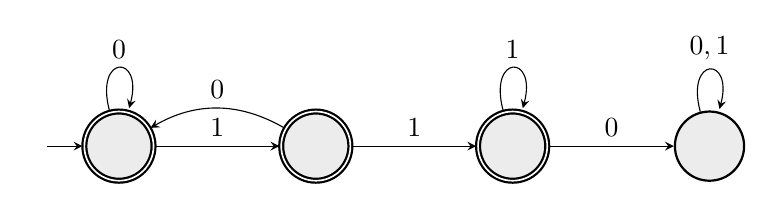
\begin{tikzpicture}
                            \node[state, accepting, initial] (q1) {};
                            \node[state, accepting, right of=q1] (q2) {};
                            \node[state, accepting, right of=q2] (q3) {};
                            \node[state, right of=q3] (q4) {};
                            \draw
                            (q1) edge[above] node{$1$} (q2)
                            (q1) edge[loop above] node{$0$} (q1)
                            (q2) edge[above] node{$1$} (q3)
                            (q2) edge[bend right, above] node{$0$} (q1)
                            (q3) edge[above] node{$0$} (q4)
                            (q3) edge[loop above] node{$1$} (q3)
                            (q4) edge[loop above] node{$0,1$} (q4);
                        \end{tikzpicture}
                    \end{figure}
              \item $\{w|\text{the length of }w\text{ is at most }5\}$

                    \begin{figure}[H]
                        \centering
                        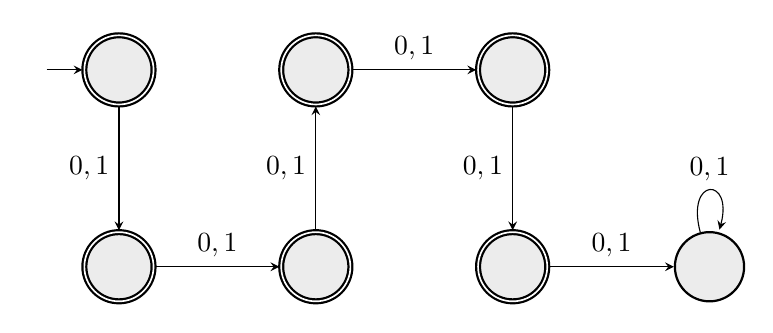
\begin{tikzpicture}
                            \node[state, accepting, initial] (q1) {};
                            \node[state, accepting, below of=q1] (q2) {};
                            \node[state, accepting, right of=q2] (q3) {};
                            \node[state, accepting, above of=q3] (q4) {};
                            \node[state, accepting, right of=q4] (q5) {};
                            \node[state, accepting, below of=q5] (q6) {};
                            \node[state, right of=q6] (q7) {};
                            \draw
                            (q7) edge[loop above] node{$0,1$} (q7)
                            (q1) edge[left] node{$0,1$} (q2)
                            (q2) edge[above] node{$0,1$} (q3)
                            (q3) edge[left] node{$0,1$} (q4)
                            (q4) edge[above] node{$0,1$} (q5)
                            (q5) edge[left] node{$0,1$} (q6)
                            (q6) edge[above] node{$0,1$} (q7);
                        \end{tikzpicture}
                    \end{figure}

              \item $\{w|w~ \text{is any string except }11\text{ and }111\}$
                    \begin{figure}[H]
                        \centering
                        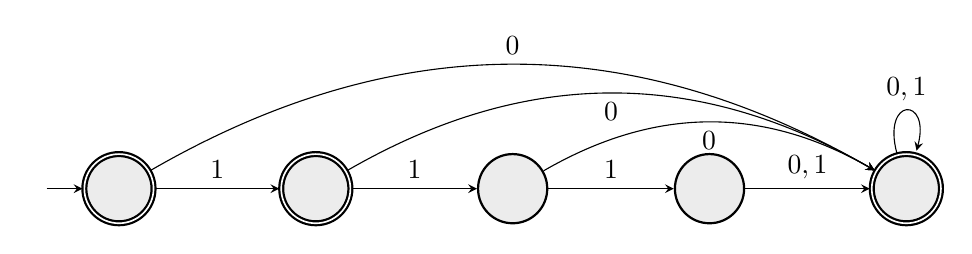
\begin{tikzpicture}
                            \node[state, accepting, initial] (q1) {};
                            \node[state, accepting, right of=q1] (q2) {};
                            \node[state, right of=q2] (q3) {};
                            \node[state, right of=q3] (q4) {};
                            \node[state, accepting, right of=q4] (q5) {};
                            \draw
                            (q1) edge[above] node{$1$} (q2)
                            (q1) edge[bend left, above] node{$0$} (q5)
                            (q2) edge[above] node{$1$} (q3)
                            (q2) edge[bend left, below ] node{$0$} (q5)
                            (q3) edge[above] node{$1$} (q4)
                            (q3) edge[bend left, below] node{$0$} (q5)
                            (q4) edge[above] node{$0,1$} (q5)
                            (q5) edge[loop above] node{$0,1$} (q5);
                        \end{tikzpicture}
                    \end{figure}
              \item $\{w|\text{ every odd position of }w\text{ is a }1\}$
                    \begin{figure}[H]
                        \centering
                        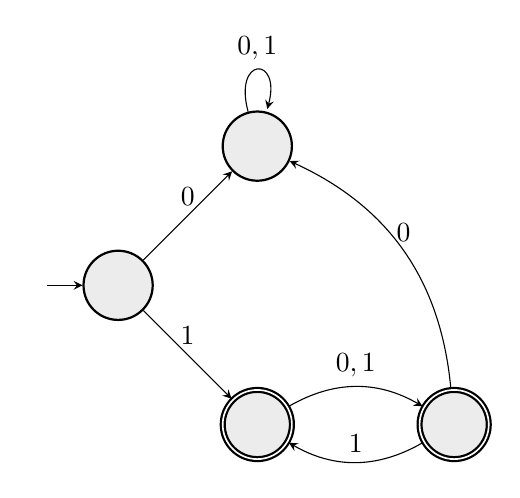
\begin{tikzpicture}
                            \node[state, initial] (q1) {};
                            \node[state, above right of=q1] (q2) {};
                            \node[state, accepting, below right of=q1] (q3) {};
                            \node[state, accepting, right of=q3] (q5) {};
                            \draw
                            (q1) edge[above] node{$0$} (q2)
                            (q1) edge[above] node{$1$} (q3)
                            (q2) edge[loop above] node{$0,1$} (q2)
                            (q3) edge[bend left, above] node{$0,1$} (q5)
                            (q5) edge[bend left, above] node{$1$} (q3)
                            (q5) edge[bend right, above] node{$0$} (q2);
                        \end{tikzpicture}
                    \end{figure}
              \item $\{w|w~ \text{contains at least two }0\text{'s and at most one }1\}$
                    \begin{figure}[H]
                        \centering
                        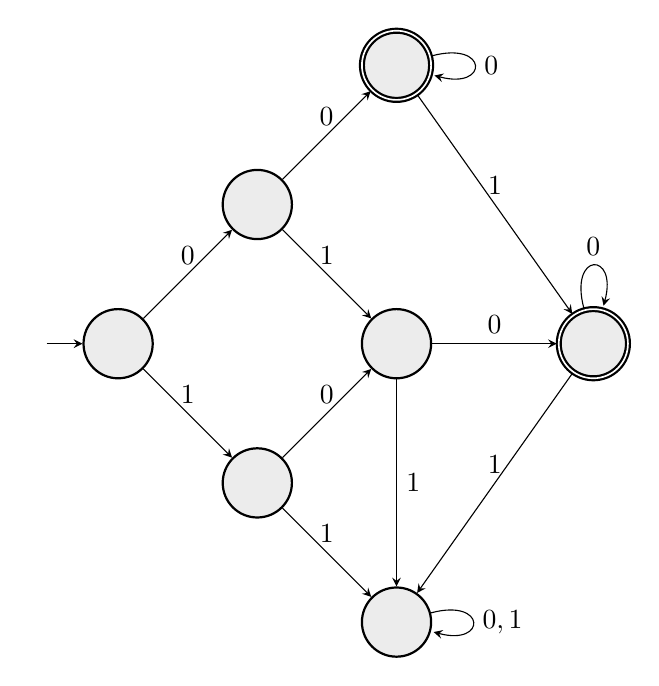
\begin{tikzpicture}
                            \node[state, initial] (q1) {};
                            \node[state, above right of=q1] (q2) {};
                            \node[state, below right of=q1] (q3) {};
                            \node[state, below right of=q2] (q4) {};
                            \node[state, accepting, above right of=q2] (q5) {};
                            \node[state, below right of=q3] (q8) {};
                            \node[state, accepting, right of=q4] (q6) {};
                            \draw
                            (q1) edge[above] node{$0$} (q2)
                            (q1) edge[above] node{$1$} (q3)
                            (q2) edge[above] node{$0$} (q5)
                            (q2) edge[above] node{$1$} (q4)
                            (q3) edge[above] node{$0$} (q4)
                            (q3) edge[above] node{$1$} (q8)
                            (q4) edge[above] node{$0$} (q6)
                            (q4) edge[right] node{$1$} (q8)
                            (q5) edge[above] node{$1$} (q6)
                            (q5) edge[loop right] node{$0$} (q5)
                            (q6) edge[loop above] node{$0$} (q6)
                            (q8) edge[loop right] node{$0,1$} (q8)
                            (q6) edge[above] node{$1$} (q8);
                        \end{tikzpicture}
                    \end{figure}
              \item $\{\epsilon,0\}$
                    \begin{figure}[H]
                        \centering
                        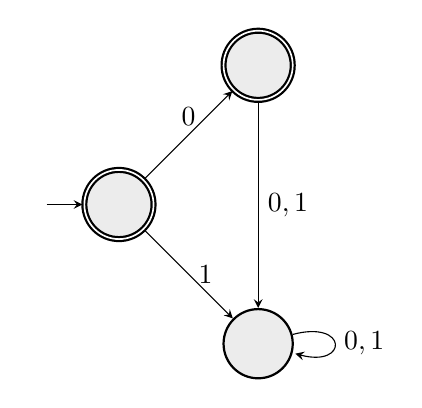
\begin{tikzpicture}
                            \node[state, initial, accepting] (q1) {};
                            \node[state, accepting, above right of=q1] (q2) {};
                            \node[state, below right of=q1] (q3) {};
                            \draw
                            (q1) edge[above] node{$0$} (q2)
                            (q1) edge[right] node{$1$} (q3)
                            (q2) edge[right] node{$0,1$} (q3)
                            (q3) edge[loop right] node{$0,1$} (q3);
                        \end{tikzpicture}
                    \end{figure}
              \item $\{w|w~ \text{contains an even number of }0\text{'s, or contains exactly two }1\text{'s}\}$
                    \begin{figure}[H]
                        \centering
                        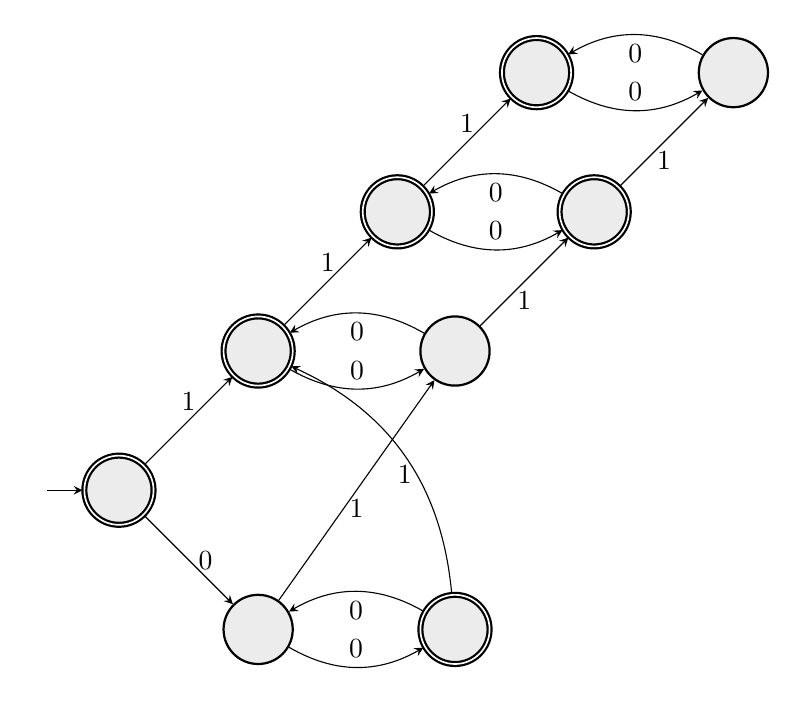
\begin{tikzpicture}
                            \node[state, initial, accepting] (q1) {};
                            \node[state, accepting, above right of=q1] (q2) {};
                            \node[state, below right of=q1] (q3) {};
                            \node[state, accepting, right of=q3] (q4) {};
                            \node[state, right of=q2] (q5) {};
                            \node[state, accepting, above right of=q2] (q6) {};
                            \node[state, accepting, right of=q6] (q7) {};
                            \node[state, accepting, above right of=q6] (q8) {};
                            \node[state, right of=q8] (q9) {};
                            \draw
                            (q1) edge[above] node{$1$} (q2)
                            (q1) edge[right] node{$0$} (q3)
                            (q3) edge[below] node{$1$} (q5)
                            (q4) edge[bend right, below] node{$1$} (q2)
                            (q3) edge[bend right, above] node{$0$} (q4)
                            (q4) edge[bend right, below] node{$0$} (q3)
                            (q2) edge[bend right, above] node{$0$} (q5)
                            (q2) edge[right, above] node{$1$} (q6)
                            (q5) edge[right, below] node{$1$} (q7)
                            (q5) edge[bend right, below] node{$0$} (q2)
                            (q6) edge[bend right, above] node{$0$} (q7)
                            (q7) edge[bend right, below] node{$0$} (q6)
                            (q6) edge[right, above] node{$1$} (q8)
                            (q7) edge[right, below] node{$1$} (q9)
                            (q8) edge[bend right, above] node{$0$} (q9)
                            (q9) edge[bend right, below] node{$0$} (q8);
                        \end{tikzpicture}
                    \end{figure}
              \item The empty set
                    \begin{figure}[H]
                        \centering
                        \begin{tikzpicture}
                            \node[state, initial] (q1) {};
                            \draw
                            (q1) edge[loop right] node{$0,1$} (q1);
                        \end{tikzpicture}
                    \end{figure}
              \item All strings except the empty string
                    \begin{figure}[H]
                        \centering
                        \begin{tikzpicture}
                            \node[state, initial] (q1) {};
                            \node[state, accepting, right of=q1] (q2) {};
                            \draw
                            (q1) edge[above] node{$0,1$} (q2)
                            (q2) edge[loop above] node{$0,1$} (q2);
                        \end{tikzpicture}
                    \end{figure}
          \end{enumerate}
\end{enumerate}

\begin{enumerate}
    \item[1.7]
          Give state diagrams of NFAs with the specified number of states recognizing each of the following languages. In all parts, the alphabet is {0,1}.
          \begin{enumerate}
              \item The language $\{w|w~ \text{ends with }00\}$ with three states
                    \begin{figure}[H]
                        \centering
                        \begin{tikzpicture}
                            \node[state, initial] (q1) {};
                            \node[state, right of=q1] (q2) {};
                            \node[state, accepting, right of=q2] (q3) {};
                            \draw
                            (q1) edge[above] node{$0$} (q2)
                            (q2) edge[above] node{$0$} (q3)
                            (q1) edge[loop above] node{$0,1$} (q1);
                        \end{tikzpicture}
                    \end{figure}
              \item The language of Exercise 1.6c with five states
                    \begin{figure}[H]
                        \centering
                        \begin{tikzpicture}
                            \node[state, initial] (q1) {};
                            \node[state, right of=q1] (q2) {};
                            \node[state, right of=q2] (q3) {};
                            \node[state, right of=q3] (q4) {};
                            \node[state, accepting, right of=q4] (q5) {};
                            \draw
                            (q1) edge[loop above] node{$1$} (q1)
                            (q1) edge[above] node{$0$} (q2)
                            (q2) edge[loop above] node{$0$} (q2)
                            (q2) edge[above] node{$1$} (q3)
                            (q3) edge[above] node{$0$} (q4)
                            (q4) edge[above] node{$1$} (q5)
                            (q5) edge[loop above] node{$0,1$} (q5)
                            (q3) edge[bend left, below] node{$1$} (q1)
                            (q4) edge[bend right, above] node{$0$} (q2);
                        \end{tikzpicture}
                    \end{figure}
              \item The language of Exercise 1.6l with six states
                    \begin{figure}[H]
                        \centering
                        \begin{tikzpicture}
                            \node[state, accepting, initial] (q1) {};
                            \node[state, above right of=q1] (q2) {};
                            \node[state, accepting, below right of=q1] (q3) {};
                            \node[state, right of=q3] (q4) {};
                            \node[state, right of=q2] (q5) {};
                            \node[state, accepting, right of=q5] (q6) {};
                            \draw
                            (q1) edge[right] node{$\epsilon$} (q2)
                            (q1) edge[above] node{$1$} (q3)
                            (q3) edge[above] node{$1$} (q4)
                            (q1) edge[loop above] node{$0$} (q1)
                            (q3) edge[loop above] node{$0$} (q3)
                            (q4) edge[loop above] node{$0$} (q4)
                            (q2) edge[loop above] node{$0,1$} (q2)
                            (q5) edge[loop above] node{$1$} (q5)
                            (q6) edge[loop above] node{$0,1$} (q6)
                            (q2) edge[right, below] node{$0$} (q5)
                            (q5) edge[right, below] node{$0$} (q6);
                        \end{tikzpicture}
                    \end{figure}
              \item The language $\{0\}$ with two states
                    \begin{figure}[H]
                        \centering
                        \begin{tikzpicture}
                            \node[state, initial] (q1) {};
                            \node[state, accepting, right of=q1] (q2) {};
                            \draw
                            (q1) edge[above] node{$0$} (q2);
                        \end{tikzpicture}
                    \end{figure}
              \item The language $0^\ast1^\ast0+$ with three states
                    \begin{figure}[H]
                        \centering
                        \begin{tikzpicture}
                            \node[state, initial] (q1) {};
                            \node[state, right of=q1] (q2) {};
                            \node[state, accepting, right of=q2] (q3) {};
                            \draw
                            (q1) edge[above] node{$\epsilon$} (q2)
                            (q2) edge[above] node{$0$} (q3)
                            (q1) edge[loop above] node{$0$} (q1)
                            (q2) edge[loop above] node{$1$} (q2)
                            (q3) edge[loop above] node{$0$} (q3);
                        \end{tikzpicture}
                    \end{figure}
              \item The language $1^\ast(001+)^\ast$ with three states
                    \begin{figure}[H]
                        \centering
                        \begin{tikzpicture}
                            \node[state, accepting, initial] (q1) {};
                            \node[state, right of=q1] (q2) {};
                            \node[state, below right of=q1] (q3) {};
                            \draw
                            (q1) edge[above] node{$0$} (q2)
                            (q2) edge[right] node{$0$} (q3)
                            (q3) edge[left] node{$1$} (q1)
                            (q1) edge[loop above] node{$1$} (q1);
                        \end{tikzpicture}
                    \end{figure}
              \item The language ${\epsilon}$ with one state
                    \begin{figure}[H]
                        \centering
                        \begin{tikzpicture}
                            \node[state, initial, accepting] (q1) {};
                        \end{tikzpicture}
                    \end{figure}
              \item The language $0^\ast$ with one state
                    \begin{figure}[H]
                        \centering
                        \begin{tikzpicture}
                            \node[state, initial, accepting] (q1) {};
                            \draw
                            (q1) edge[loop above] node{$0$} (q1);
                        \end{tikzpicture}
                    \end{figure}
          \end{enumerate}
    \item[1.8]
          Use the construction in the proof of Theorem 1.45 to give the state diagrams of NFAs recognizing the union of the languages described in:
          \begin{enumerate}
              \item  Exercises 1.6a and 1.6b
                    \begin{figure}[H]
                        \centering
                        \begin{tikzpicture}
                            \node[state, initial] (q0) {};
                            \node[state, above right of=q0] (q1) {};
                            \node[state, right of=q1] (q2) {};
                            \node[state, accepting, right of=q2] (q3) {};
                            \node[state, right of=q3] (q4) {};
                            \node[state, below right of=q0] (bq1) {};
                            \node[state, right of=bq1] (bq2) {};
                            \node[state, right of=bq2] (bq3) {};
                            \node[state, accepting, right of=bq3] (bq4) {};
                            \draw
                            (q0) edge[above, blue] node{$\epsilon$} (q1)
                            (q0) edge[above, blue] node{$\epsilon$} (bq1)
                            (q1) edge[above] node{$1$} (q2)
                            (q2) edge[loop above] node{$1$} (q2)
                            (q2) edge[bend left, above] node{$0$} (q3)
                            (q3) edge[loop above] node{$0$} (q3)
                            (q3) edge[bend left, below] node{$1$} (q2)
                            (q1) edge[bend right, below] node{$0$} (q4)
                            (q4) edge[loop above] node{$0,1$} (q4)
                            (q1) edge[loop above] node{$0$} (q1)
                            (bq1) edge[above] node{$1$} (bq2)
                            (bq2) edge[loop above] node{$0$} (bq2)
                            (bq2) edge[above] node{$1$} (bq3)
                            (bq3) edge[loop above] node{$0$} (bq3)
                            (bq3) edge[above] node{$1$} (bq4)
                            (bq4) edge[loop above] node{$0,1$} (bq4);
                        \end{tikzpicture}
                    \end{figure}
              \item Exercises 1.6c and 1.6f
                    \begin{figure}[H]
                        \centering
                        \begin{tikzpicture}
                            \node[state, initial] (q0) {};
                            \node[state, above right of=q0] (q1) {};
                            \node[state, right of=q1] (q2) {};
                            \node[state, right of=q2] (q3) {};
                            \node[state, right of=q3] (q4) {};
                            \node[state, accepting, right of=q4] (q5) {};
                            \node[state, accepting, below right of=q0] (bq1) {};
                            \node[state, accepting, right of=bq1] (bq2) {};
                            \node[state, accepting, right of=bq2] (bq3) {};
                            \node[state, right of=bq3] (bq4) {};
                            \draw
                            (q0) edge[above, blue] node{$\epsilon$} (q1)
                            (q0) edge[above, blue] node{$\epsilon$} (bq1)
                            (q1) edge[loop above] node{$1$} (q1)
                            (q1) edge[above] node{$0$} (q2)
                            (q2) edge[loop above] node{$0$} (q2)
                            (q2) edge[above] node{$1$} (q3)
                            (q3) edge[above] node{$0$} (q4)
                            (q4) edge[above] node{$1$} (q5)
                            (q5) edge[loop above] node{$0,1$} (q5)
                            (q3) edge[bend left, below] node{$1$} (q1)
                            (q4) edge[bend right, above] node{$0$} (q2)
                            (bq1) edge[above] node{$1$} (bq2)
                            (bq1) edge[loop above] node{$0$} (bq1)
                            (bq2) edge[above] node{$1$} (bq3)
                            (bq2) edge[bend right, above] node{$0$} (bq1)
                            (bq3) edge[above] node{$0$} (bq4)
                            (bq3) edge[loop above] node{$1$} (bq3)
                            (bq4) edge[loop above] node{$0,1$} (bq4);
                        \end{tikzpicture}
                    \end{figure}
          \end{enumerate}
    \item[1.9]
          Use the construction in the proof of Theorem 1.47 to give the state diagrams of NFAs recognizing the concatenation of the languages described in
          \begin{enumerate}
              \item Exercises 1.6g and 1.6i.
                    \begin{figure}[H]
                        \centering
                        \begin{tikzpicture}
                            \node[state, accepting, initial] (q1) {};
                            \node[state, accepting, below of=q1] (q2) {};
                            \node[state, accepting, right of=q2] (q3) {};
                            \node[state, accepting, above of=q3] (q4) {};
                            \node[state, accepting, right of=q4] (q5) {};
                            \node[state, accepting, below of=q5] (q6) {};
                            \node[state, right of=q6] (q7) {};
                            \node[state, below of=q7] (bq1) {};
                            \node[state, above right of=bq1] (bq2) {};
                            \node[state, accepting, below right of=bq1] (bq3) {};
                            \node[state, accepting, right of=bq3] (bq5) {};
                            \draw
                            (q7) edge[loop above] node{$0,1$} (q7)
                            (q1) edge[left] node{$0,1$} (q2)
                            (q2) edge[above] node{$0,1$} (q3)
                            (q3) edge[left] node{$0,1$} (q4)
                            (q4) edge[above] node{$0,1$} (q5)
                            (q5) edge[left] node{$0,1$} (q6)
                            (q6) edge[above] node{$0,1$} (q7)
                            
                            (bq1) edge[above] node{$0$} (bq2)
                            (bq1) edge[above] node{$1$} (bq3)
                            (bq2) edge[loop above] node{$0,1$} (bq2)
                            (bq3) edge[bend left, above] node{$0,1$} (bq5)
                            (bq5) edge[bend left, above] node{$1$} (bq3)
                            (bq5) edge[bend right, above] node{$0$} (bq2)
                            
                            (q1) edge[left, below, blue] node{$\epsilon$} (bq1)
                            (q2) edge[left, below, blue] node{$\epsilon$} (bq1)
                            (q3) edge[left, below, blue] node{$\epsilon$} (bq1)
                            (q4) edge[left, below, blue] node{$\epsilon$} (bq1)
                            (q5) edge[left, below, blue] node{$\epsilon$} (bq1);
                        \end{tikzpicture}
                    \end{figure}
              \item Exercises 1.6b and 1.6m.
                    \begin{figure}[H]
                        \centering
                        \begin{tikzpicture}
                            \node[state, initial] (q1) {};
                            \node[state, right of=q1] (q2) {};
                            \node[state, right of=q2] (q3) {};
                            \node[state, accepting, right of=q3] (q4) {};
                            \node[state, right of=q4] (bq1) {};
                            \draw
                            (q1) edge[loop above] node{$0$} (q1)
                            (q1) edge[above] node{$1$} (q2)
                            (q2) edge[loop above] node{$0$} (q2)
                            (q2) edge[above] node{$1$} (q3)
                            (q3) edge[loop above] node{$0$} (q3)
                            (q3) edge[above] node{$1$} (q4)
                            (q4) edge[loop above] node{$0,1$} (q4)
                            (q4) edge[above, blue] node{$\epsilon$} (bq1)
                            (bq1) edge[loop right] node{$0,1$} (bq1);
                        \end{tikzpicture}
                    \end{figure}
          \end{enumerate}
          
    \item [1.10]
          Use the construction in the proof of Theorem 1.49 to give the state diagrams of NFAs recognizing the star of the languages described in 
          \begin{enumerate}
              \item Exercise 1.6b.
                    \begin{figure}[H]
                        \centering
                        \begin{tikzpicture}
                            \node[state, accepting, initial] (q0) {};
                            \node[state, right of=q0] (q1) {};
                            \node[state, right of=q1] (q2) {};
                            \node[state, right of=q2] (q3) {};
                            \node[state, accepting, right of=q3] (q4) {};
                            \draw
                            (q0) edge[above] node{$\epsilon$} (q1)
                            
                            (q1) edge[loop above] node{$0$} (q1)
                            (q1) edge[above] node{$1$} (q2)
                            (q2) edge[loop above] node{$0$} (q2)
                            (q2) edge[above] node{$1$} (q3)
                            (q3) edge[loop above] node{$0$} (q3)
                            (q3) edge[above] node{$1$} (q4)
                            (q4) edge[loop above] node{$0,1$} (q4)
                            
                            (q4) edge[bend left, below] node{$\epsilon$} (q1);
                        \end{tikzpicture}
                    \end{figure}
              \item Exercise 1.6j.
                    \begin{figure}[H]
                        \centering
                        \begin{tikzpicture}
                            \node[state, initial] (q0) {};
                            \node[state, right of=q0] (q1) {};
                            \node[state, above right of=q1] (q2) {};
                            \node[state, below right of=q1] (q3) {};
                            \node[state, below right of=q2] (q4) {};
                            \node[state, accepting, above right of=q2] (q5) {};
                            \node[state, below right of=q3] (q8) {};
                            \node[state, accepting, right of=q4] (q6) {};
                            \draw
                            (q0) edge[above] node{$\epsilon$} (q1)
                            (q1) edge[above] node{$0$} (q2)
                            (q1) edge[above] node{$1$} (q3)
                            (q2) edge[above] node{$0$} (q5)
                            (q2) edge[above] node{$1$} (q4)
                            (q3) edge[above] node{$0$} (q4)
                            (q3) edge[above] node{$1$} (q8)
                            (q4) edge[above] node{$0$} (q6)
                            (q4) edge[right] node{$1$} (q8)
                            (q5) edge[above] node{$1$} (q6)
                            (q5) edge[loop right] node{$0$} (q5)
                            (q6) edge[loop above] node{$0$} (q6)
                            (q8) edge[loop right] node{$0,1$} (q8)
                            (q6) edge[above] node{$1$} (q8)
                            
                            (q5) edge[bend left, below] node{$\epsilon$} (q1)
                            (q6) edge[bend left, below] node{$\epsilon$} (q1);
                        \end{tikzpicture}
                    \end{figure}
              \item Exercise 1.6m.
                    \begin{figure}[H]
                        \centering
                        \begin{tikzpicture}
                            \node[state, initial, accepting] (q0) {};
                            \node[state, right of=q0] (q1) {};
                            \draw
                            (q0) edge[above] node{$\epsilon$} (q1)
                            (q1) edge[loop right] node{$0,1$} (q1);
                        \end{tikzpicture}
                    \end{figure}
          \end{enumerate}
          
    \item [1.11]
          Prove that every NFA can be converted to an equivalent one that has a single accept state.
          
          It is enough to show that every NFA can be converted to an equivalent one that has a single accept state and no transitions into the accept state. Let $N = (Q, \Sigma, \delta, q_0, F)$ be an NFA. We construct an NFA $N' = (Q \cup \{q_f\}, \Sigma, \delta', q_0, \{q_f\})$ where $\delta'$ is the same as $\delta$ with additional transitions: for each $q \in F$ $\delta'(q, \epsilon) = \{q_f\}$. It is clear that $L(N) = L(N')$ and that $N'$ has a single accept state. Therefore, every NFA can be converted to an equivalent one that has a single accept state.
          
    \item [1.12]
          
          Let \[D = \{w|w~ \text{contains an even number of }a\text{’s and an odd number of }b\text{’s}\]
          \[ \text{and does not contain the substring }ab\}\] Give a DFA with five states that recognizes $D$ and a regular expression that generates $D$. (Suggestion: Describe $D$ more simply.)
          
          $$D = \{w|w~ \text{contains odd number of }b\text{'s followed by even number of }a\text{'s} \}$$
          
          \begin{figure}[H]
              \centering
              \begin{tikzpicture}
                  \node[state, initial] (q0) {};
                  \node[state, accepting, right of=q0] (q1) {};
                  \node[state, right of=q1] (q2) {};
                  \node[state, right of=q2] (q3) {};
                  \node[state, above of=q1] (q5) {};
                  \draw
                  (q0) edge[above] node{$b$} (q1)
                  (q0) edge[bend right, below] node{$a$} (q2)
                  (q1) edge[bend left, left] node{$b$} (q5)
                  (q5) edge[bend left, left] node{$b$} (q1)
                  (q1) edge[bend left, below] node{$a$} (q2)
                  (q2) edge[bend left, above] node{$a$} (q1)
                  (q2) edge[below] node{$b$} (q3)
                  (q5) edge[below] node{$a$} (q3)
                  (q3) edge[loop above] node{$a,b$} (q3);
              \end{tikzpicture}
          \end{figure}
          
          The regular expression that generates $D$ is $b(bb)^{\ast}(aa)^{\ast}$.
\end{enumerate}

\begin{enumerate}

    \item [1.13]
          
          Let $F$ be the language of all strings over $\{0,1\}$ that do not contain a pair of $1$s that are separated by an odd number of symbols. Give the state diagram of a DFA with five states that recognizes $F$. (You may find it helpful first to find a 4-state NFA for the complement of $F$.) blab
          
          $\overline{F} = \{w|w~ \text{contains a pair of }1\text{'s that are separated by an odd number of symbols}\}$
          
          \begin{figure}[H]
              \centering
              \begin{tikzpicture}
                  \node[state, initial] (q0) {};
                  \node[state, right of=q0] (q1) {};
                  \node[state, above of=q1] (q2) {};
                  \node[state, accepting, right of=q1] (q3) {};
                  \draw
                  (q0) edge[above] node{$1$} (q1)
                  (q0) edge[bend right, below] node{$1$} (q2)
                  (q2) edge[above] node{$1$} (q3)
                  (q2) edge[bend right, above] node{$1$} (q3)
                  (q3) edge[loop above] node{$0$} (q3);
              \end{tikzpicture}
              \caption{NFA with four states that recognizes $\overline{F}$}
          \end{figure}
    \item [1.14]
          \begin{enumerate}
              \item Show that if $M$ is a DFA that recognizes language $B$, swapping the accept and nonaccept states in $M$ yields a new DFA recognizing the complement of $B$.Conclude that the class of regular languages is closed under complement.
                    
                    Every state in DFA has a transition for every symbol in the alphabet. For every possible word, the DFA will end up in either an accept state or a nonaccept state. If we swap the accept and nonaccept states in $M$, the new DFA will accept the complement of the language $B$.
                    
              \item Show by giving an example that if $M$ is an NFA that recognizes language $C$, swapping the accept and non-accept states in $M$ doesn’t necessarily yield a new NFA that recognizes the complement of $C$. Is the class of languages recognized by NFAs closed under complement? Explain your answer.
                    
                    \begin{figure}[H]
                        \centering
                        \begin{tikzpicture}
                            \node[state, initial] (q0) {};
                            \node[state, accepting, right of=q0] (q1) {};
                            \draw
                            (q0) edge[above] node{$0,1$} (q1)
                            (q0) edge[loop above] node{$0$} (q0);
                        \end{tikzpicture}
                        \caption{example NFA}
                        \begin{tikzpicture}
                            \node[state, accepting, initial] (q0) {};
                            \node[state, right of=q0] (q1) {};
                            \draw
                            (q0) edge[above] node{$0,1$} (q1)
                            (q0) edge[loop above] node{$0$} (q0);
                        \end{tikzpicture}
                        \caption{example NFA with changed states acceptance}
                    \end{figure}
                    
                    NFA accepts a string if there is at least one path that leads to an accept state. If we swap the accept and non-accept states in $M$, the new NFA will not necessarily accept the complement of the language $C$. The class of languages recognized by NFAs is not closed under complement.
          \end{enumerate}
    \item [1.15]
          Give a counter example to show that the following construction fails to prove Theorem 1.49, the closure of the class of regular languages under the star operation. Let $N_1 = (Q_1,\Sigma,\delta_1,q_1,F_1)$ recognize $A_1$. Construct $N = (Q_1,\Sigma,\delta,q_1,F)$ as follows. $N$ is supposed to recognize $A_1^\ast$.
          \begin{enumerate}
              \item The states of $N$ are the states of $N_1$.
              \item The start state of $N$ is the same as the start state of $N_1$.
              \item $F =\{q_1\} \cup F_1$.
                    
                    The accept states F are the old accept states plus its start state.
              \item Define $\delta$ so that for any $q \in Q_1$ and any $a \in \Sigma_\epsilon$,
                    $$\delta(q,a)=
                        \begin{cases}
                            \delta_1(q,a)              & q \notin F_1~ \text{or }a \neq \epsilon \\
                            \delta_1(q,a) \cup \{q_1\} & q \in F_1~ \text{and }a = \epsilon.
                        \end{cases}
                    $$
          \end{enumerate}
          (Suggestion: Show this construction graphically, as in Figure 1.50.)
          
          \begin{figure}[H]
              \centering
              \begin{tikzpicture}

                  \node[state, initial] (q0) {};
                  \node[state, right of=q0, minimum size=0.5cm] (q02) {};
                  \node[state, above of=q02, minimum size=0.5cm] (q01) {};
                  \node[state, below of=q02, minimum size=0.5cm] (q03) {};
                  \node[state, accepting, above right of=q02] (q2) {};
                  \node[state, accepting, below of=q2] (q3) {};
              \end{tikzpicture}
              \caption{NFA $N_1$}
          \end{figure}
          \begin{figure}[H]
              \centering
              \begin{tikzpicture}
                  \node[state, accepting, initial] (q0) {};
                  \node[state, right of=q0, minimum size=0.5cm] (q02) {};
                  \node[state, above of=q02, minimum size=0.5cm] (q01) {};
                  \node[state, below of=q02, minimum size=0.5cm] (q03) {};
                  \node[state, accepting, above right of=q02] (q2) {};
                  \node[state, accepting, below of=q2] (q3) {};
                  \draw
                  (q2) edge[bend right, above] node{$\epsilon$} (q0)
                  (q3) edge[bend left, above] node{$\epsilon$} (q0);
              \end{tikzpicture}
              \caption{construction of NFA $N_1$}
          \end{figure}
          
          \begin{figure}[H]
              \centering
              \begin{tikzpicture}
                  \node[state, initial] (q0) {};
                  \node[state, accepting, right of=q0] (q1) {};
                  \draw
                  (q0) edge[bend right, above] node{$0$} (q1)
                  (q1) edge[bend right, above] node{$1$} (q0);
              \end{tikzpicture}
              \caption{counter example of NFA $N_1$}
          \end{figure}
    \item [1.16]
          Use the construction given in Theorem 1.39 to convert the following two nondeterministic finite automata to equivalent deterministic finite automata.
          \begin{enumerate}
              \item
              
                    \begin{figure}[H]
                        \centering
                        \begin{tikzpicture}
                            \node[state, accepting, initial] (q1) {$1$};
                            \node[state, below of=q0] (q2) {$2$};
                            \draw
                            (q1) edge[bend right, left] node{$a,b$} (q2)
                            (q2) edge[bend right, right] node{$b$} (q1)
                            (q1) edge[loop right] node{$a$} (q1);
                        \end{tikzpicture}
                        \caption{NFA $A$}
                    \end{figure}
                    $A^\prime = (Q^\prime, \Sigma, \delta^\prime, \{1\}, F^\prime)$
                    
                    $Q^\prime = \{\emptyset,\{1\},\{2\},\{1,2\}\}$
                    
                    $\Sigma = \{a,b\}$
                    
                    $F^\prime = \{\{1\},\{1,2\}\}$
                    
                    \begin{figure}[H]
                        \centering
                        \begin{tikzpicture}
                            \node[state, accepting, initial] (q1) {$\{1\}$};
                            \node[state, below of=q0] (q2) {$\{2\}$};
                            \node[state, below of=q2] (q3) {$\emptyset$};
                            \node[state, accepting, right of=q2] (q4) {$\{1,2\}$};
                            \draw
                            (q1) edge[bend right, left] node{$b$} (q2)
                            (q2) edge[bend left, left] node{$a$} (q3)
                            (q3) edge[loop left] node{$a,b$} (q3)
                            (q1) edge[loop right] node{$a$} (q1)
                            (q4) edge[loop right] node{$a,b$} (q4)
                            (q2) edge[bend right, right] node{$b$} (q1);
                        \end{tikzpicture}
                        \caption{DFA $A^\prime$}
                    \end{figure}
              \item
                    \begin{figure}[H]
                        \centering
                        \begin{tikzpicture}
                            \node[state, initial] (q1) {$1$};
                            \node[state, accepting, right of=q1] (q2) {$2$};
                            \node[state, below left of=q2] (q3) {$3$};
                            \draw
                            (q1) edge[bend right, above] node{$\epsilon$} (q2)
                            (q1) edge[bend right, right] node{$a$} (q3)
                            (q2) edge[bend right, above] node{$a$} (q1)
                            (q3) edge[bend right, right] node{$a,b$} (q2)
                            (q3) edge[loop right] node{$b$} (q3);
                        \end{tikzpicture}
                        \caption{NFA $B$}
                    \end{figure}
                    $B^\prime = (Q^\prime, \Sigma, \delta^\prime, \{1\}, F^\prime)$
                    
                    $Q^\prime = \{\emptyset,\{1\},\{2\},\{3\},\{1,2\},\{1,3\},\{2,3\},\{1,2,3\}\}$
                    
                    $\Sigma = \{a,b\}$
                    
                    $F^\prime = \{\{2\},\{1,2\},\{2,3\},\{1,2,3\}\}$
                    
                    \begin{figure}[H]
                        \centering
                        \begin{tikzpicture}
                            \node[state] (q1) {$\{1\}$};
                            \node[state, accepting, right of=q1] (q2) {$\{2\}$};
                            
                            \node[state, accepting, below right of=q2, initial] (q12) {$\{1,2\}$};
                            \node[state, below left of=q12] (q0) {$\emptyset$};
                            
                            \node[state, right of=q12] (q13) {$\{1,3\}$};
                            \node[state, above of=q13] (q3) {$\{3\}$};
                            \node[state, accepting, right of=q13] (q23) {$\{2,3\}$};
                            \node[state, accepting, right of=q23] (q123) {$\{1,2,3\}$};
                            \draw
                            (q1) edge[bend left=40, above] node{$a$} (q123)
                            (q1) edge[bend right, left] node{$b$} (q0)
                            (q2) edge[right, below left] node{$b$} (q0)
                            (q2) edge[bend right, above] node{$a$} (q12)
                            (q3) edge[bend left, above right] node{$b$} (q23)
                            (q3) edge[above] node{$a$} (q2)
                            
                            (q12) edge[bend right=60, below] node{$a$} (q123)
                            (q12) edge[right, below] node{$b$} (q0)
                            
                            (q23) edge[bend left, below] node{$a$} (q12)
                            (q23) edge[loop above] node{$b$} (q23)
                            (q123) edge[bend right, above] node{$b$} (q23)
                            
                            (q13) edge[right, below] node{$a,b$} (q23)
                            
                            (q123) edge[loop right] node{$a$} (q123);
                        \end{tikzpicture}
                        \caption{DFA $B^\prime$}
                    \end{figure}
          \end{enumerate}
    \item [1.17]
          \begin{enumerate}
              \item Give an NFA recognizing the language $(01 \cup 001 \cup 010)^\ast$
                    \begin{figure}[H]
                        \centering
                        \begin{tikzpicture}
                            \node[state, initial] (q0) {};
                            \node[state, right of=q0] (q2) {};
                            \node[state, above right of=q2] (q11) {};
                            
                            \node[state, right of=q2] (q21) {};
                            \node[state, right of=q21] (q22) {};
                            \node[state, right of=q11] (q31) {};
                            
                            \node[state, accepting, right of=q22] (qend) {};
                            \draw
                            (q0) edge[above] node{$0$} (q2)
                            (q2) edge[above] node{$1$} (q11)
                            (q2) edge[above] node{$0$} (q21)
                            (q21) edge[above] node{$1$} (q22)
                            
                            (q11) edge[above] node{$0$} (q31)
                            
                            (q11) edge[above] node{$\epsilon$} (qend)
                            (q31) edge[above] node{$\epsilon$} (qend)
                            (q22) edge[below] node{$\epsilon$} (qend)
                            (qend) edge[bend right=70, above] node{$\epsilon$} (q0);
                        \end{tikzpicture}
                        \caption{NFA recognizing the language $(01 \cup 001 \cup 010)^\ast$}
                    \end{figure}
              \item Convert this NFA to an equivalent DFA. Give only the portion of the DFA that is reachable from the start state.
                    \begin{figure}[H]
                        \centering
                        \begin{tikzpicture}
                            \node[state, initial] (q0) {};
                            \node[state, right of=q0] (q2) {};
                            \node[state, above right of=q2] (q11) {};
                            
                            \node[state, right of=q2] (q21) {};
                            \node[state, right of=q21] (q22) {};
                            \node[state, right of=q11] (q31) {};
                            
                            \node[state, accepting, right of=q22] (qend) {};
                            \draw
                            (q0) edge[above] node{$0$} (q2)
                            (q2) edge[above] node{$1$} (q11)
                            (q2) edge[above] node{$0$} (q21)
                            (q21) edge[above] node{$1$} (q22)
                            
                            (q11) edge[above] node{$0$} (q31)
                            
                            (q11) edge[above] node{$\epsilon$} (qend)
                            (q31) edge[above] node{$\epsilon$} (qend)
                            (q22) edge[below] node{$\epsilon$} (qend)
                            (qend) edge[bend right=70, above] node{$\epsilon$} (q0);
                        \end{tikzpicture}
                        \caption{DFA recognizing the language $(01 \cup 001 \cup 010)^\ast$}
                    \end{figure}
          \end{enumerate}
    \item [1.18]
          Give regular expressions generating the languages of Exercise 1.6.
          \begin{enumerate}
              \item $\{w|w~ \text{begins with a }1\text{ and ends with a }0\}$
                    \begin{align*}
                        1\Sigma^*0
                    \end{align*}
              \item $\{w|w~ \text{contains at least three }1\text{'s}\}$
                    \begin{align*}
                        \Sigma^*1\Sigma^*1\Sigma^*1\Sigma^*
                    \end{align*}
              \item $\{w|w~ \text{contains the substring }0101\}$
                    \begin{align*}
                        \Sigma^*0101\Sigma^*
                    \end{align*}
              \item $\{w|w~ \text{has length at least }3\text{ and its third symbol is a }0\}$
                    \begin{align*}
                        \Sigma\Sigma0\Sigma^*
                    \end{align*}
              \item $\{w|w~ \text{starts with }0\text{ and has odd length, or starts with }1\text{ and has even length}\}$
                    \begin{align*}
                        0(\Sigma\Sigma)^* \cup 1\Sigma(\Sigma\Sigma)^*
                    \end{align*}
              \item $\{w|w~ \text{doesn't contain the substring }110\}$
                    \begin{align*}
                        (0 \cup 10)^\ast (1 \cup 111^\ast \cup \epsilon) = 
                        (0 \cup 10)^\ast 1^\ast
                    \end{align*}
                    in details:
                    
                    \begin{figure}[H]
                        \centering
                        \begin{tikzpicture}
                            \node[state, accepting, initial] (q1) {};
                            \node[state, accepting, right of=q1] (q2) {};
                            \node[state, accepting, right of=q2] (q3) {};
                            \node[state, right of=q3] (q4) {};
                            \draw
                            (q1) edge[above] node{$1$} (q2)
                            (q1) edge[loop above] node{$0$} (q1)
                            (q2) edge[above] node{$1$} (q3)
                            (q2) edge[bend right, above] node{$0$} (q1)
                            (q3) edge[above] node{$0$} (q4)
                            (q3) edge[loop above] node{$1$} (q3)
                            (q4) edge[loop above] node{$0,1$} (q4);
                        \end{tikzpicture}
                        \caption{DFA that recognizes the language}
                    \end{figure}
                    
                    \begin{figure}[H]
                        \centering
                        \begin{tikzpicture}
                            \node[state, initial] (q0) {start};
                            \node[state, accepting, right of=q0] (q1) {A};
                            \node[state, accepting, right of=q1] (q2) {B};
                            \node[state, accepting, right of=q2] (q3) {C};
                            \node[state, right of=q3] (q4) {D};
                            \node[state, below of=q2] (qend) {acc};
                            \draw
                            (q0) edge[above] node{$\epsilon$} (q1)
                            (q1) edge[above] node{$1$} (q2)
                            (q1) edge[loop above] node{$0$} (q1)
                            (q2) edge[above] node{$1$} (q3)
                            (q2) edge[bend right, above] node{$0$} (q1)
                            (q3) edge[above] node{$0$} (q4)
                            (q3) edge[loop above] node{$1$} (q3)
                            (q4) edge[loop above] node{$0,1$} (q4)
                            (q1) edge[above] node{$\epsilon$} (qend)
                            (q2) edge[left] node{$\epsilon$} (qend)
                            (q3) edge[left] node{$\epsilon$} (qend);
                        \end{tikzpicture}
                        \caption{GNFA that recognizes the language}
                    \end{figure}
                    
                    \begin{figure}[H]
                        \centering
                        \begin{tikzpicture}
                            \node[state, initial] (q0) {start};
                            \node[state, accepting, right of=q0] (q1) {A};
                            \node[state, accepting, right of=q1] (q2) {B};
                            \node[state, accepting, right of=q2] (q3) {C};
                            \node[state, below of=q2] (qend) {acc};
                            \draw
                            (q0) edge[above] node{$\epsilon$} (q1)
                            (q1) edge[above] node{$1$} (q2)
                            (q1) edge[loop above] node{$0$} (q1)
                            (q2) edge[above] node{$1$} (q3)
                            (q2) edge[bend right, above] node{$0$} (q1)
                            (q3) edge[loop above] node{$1$} (q3)
                            (q1) edge[above] node{$\epsilon$} (qend)
                            (q2) edge[left] node{$\epsilon$} (qend)
                            (q3) edge[left] node{$\epsilon$} (qend);
                        \end{tikzpicture}
                        \caption{GNFA - removed state D}
                    \end{figure}
                    
                    \begin{figure}[H]
                        \centering
                        \begin{tikzpicture}
                            \node[state, initial] (q0) {start};
                            \node[state, accepting, right of=q0] (q1) {A};
                            \node[state, accepting, right of=q1] (q2) {B};
                            \node[state, below of=q2] (qend) {acc};
                            \draw
                            (q0) edge[above] node{$\epsilon$} (q1)
                            (q1) edge[above] node{$1$} (q2)
                            (q1) edge[loop above] node{$0$} (q1)
                            
                            (q2) edge[bend right, above] node{$0$} (q1)
                            (q2) edge[bend left, right] node{$11^\ast\epsilon$} (qend)
                            (q1) edge[above] node{$\epsilon$} (qend)
                            (q2) edge[left] node{$\epsilon$} (qend);
                        \end{tikzpicture}
                        \caption{GNFA - removed state C}
                    \end{figure}
                    
                    \begin{figure}[H]
                        \centering
                        \begin{tikzpicture}
                            \node[state, initial] (q0) {start};
                            \node[state, accepting, right of=q0] (q1) {A};
                            \node[state, right of=q1] (qend) {acc};
                            \draw
                            (q0) edge[above] node{$\epsilon$} (q1)
                            (q1) edge[loop above] node{$0 \cup 10$} (q1)
                            
                            (q1) edge[bend left, above] node{$1 \cup 111^\ast\epsilon$} (qend)
                            (q1) edge[bend right, below] node{$\epsilon$} (qend);
                        \end{tikzpicture}
                        \caption{GNFA - removed state B}
                    \end{figure}
                    
                    \begin{figure}[H]
                        \centering
                        \begin{tikzpicture}
                            [node distance=6cm]
                            \node[state, initial] (q0) {start};
                            \node[state, right of=q0] (qend) {acc};
                            \draw
                            (q0) edge[above] node{$(0 \cup 10)^\ast(1 \cup 111^\ast\epsilon \cup \epsilon)$} (qend);
                        \end{tikzpicture}
                        \caption{GNFA - removed state A}
                    \end{figure}
              \item $\{w|\text{the length of }w\text{ is at most }5\}$
                    \begin{align*}
                        (\epsilon \cup 0 \cup 1)(\epsilon \cup 0 \cup 1)(\epsilon \cup 0 \cup 1)(\epsilon \cup 0 \cup 1)(\epsilon \cup 0 \cup 1)
                    \end{align*}
              \item $\{w|w~ \text{is any string except }11\text{ and }111\}$
                    \begin{align*}
                        \epsilon \cup 0\Sigma^\ast \cup 1 \cup 10\Sigma^\ast \cup 110\Sigma^\ast \cup 1110\Sigma^\ast \cup 1111\Sigma^\ast
                    \end{align*}
              \item $\{w|\text{ every odd position of }w\text{ is a }1\}$
                    \begin{align*}
                        1((\Sigma)1)^*
                    \end{align*}
              \item $\{w|w~ \text{contains at least two }0\text{'s and at most one }1\}$
                    \begin{align*}
                        00^\ast0 \cup 100^\ast0 \cup 00^\ast10^\ast0 \cup 000^\ast1
                    \end{align*}
              \item $\{\epsilon,0\}$
                    \begin{align*}
                        \emptyset^\ast \cup 0
                    \end{align*}
              \item $\{w|w~ \text{contains an even number of }0\text{'s, or contains exactly two }1\text{'s}\}$
                    \begin{align*}
                        (1^*01^*01^*)^* \cup 0^*10^*10^*
                    \end{align*}
              \item The empty set
                    \begin{align*}
                        1\emptyset
                    \end{align*}
              \item All strings except the empty string
                    \begin{align*}
                        \Sigma\Sigma^\ast
                    \end{align*}
                    
          \end{enumerate}
\end{enumerate}

\begin{enumerate}

    \item [1.19]
          Use the procedure described in Lemma 1.55 to convert the following regular expressions to nondeterministic finite automata.
          \begin{enumerate}
              \item $(0 \cup 1)^\ast000(0 \cup 1)^\ast$
                    \begin{figure}[H]
                        \centering
                        \begin{tikzpicture}[
                                styleSmall/.style={minimum size=4mm},
                                node distance=1.5cm,
                            ]
                            \node[state, accepting, initial, styleSmall] (q01asts) {};
                            \node[state, styleSmall, right of=q01asts] (q01sum) {};
                            \node[state, above right of=q01sum, styleSmall] (q01sum0) {};
                            \node[state, accepting, right of=q01sum0, styleSmall] (q01sum00) {};
                            \node[state, below right of=q01sum, styleSmall] (q01sum1) {};
                            \node[state, accepting, right of=q01sum1, styleSmall] (q01sum11) {};
                            \draw
                            (q01asts) edge[above] node{$\epsilon$} (q01sum)
                            (q01sum) edge[above] node{$\epsilon$} (q01sum0)
                            (q01sum) edge[above] node{$\epsilon$} (q01sum1)
                            (q01sum0) edge[above] node{$0$} (q01sum00)
                            (q01sum1) edge[above] node{$1$} (q01sum11)
                            (q01sum00) edge[bend right=80, above] node{$\epsilon$} (q01sum)
                            (q01sum11) edge[bend left=80, below] node{$\epsilon$} (q01sum);
                        \end{tikzpicture}
                        \caption{$(0 \cup 1)^\ast$}
                    \end{figure}
                    \begin{figure}[H]
                        \centering
                        \begin{tikzpicture}[
                                styleSmall/.style={minimum size=4mm},
                                node distance=1.5cm,
                            ]
                            \node[state, initial, styleSmall] (q01asts) {};
                            \node[state, styleSmall, right of=q01asts] (q01sum) {};
                            \node[state, above right of=q01sum, styleSmall] (q01sum0) {};
                            \node[state, right of=q01sum0, styleSmall] (q01sum00) {};
                            \node[state, below right of=q01sum, styleSmall] (q01sum1) {};
                            \node[state, right of=q01sum1, styleSmall] (q01sum11) {};

                            \node[state, below right of=q01sum00, styleSmall] (qzs) {};
                            \node[state, right of=qzs, styleSmall] (qz0) {};
                            \node[state, right of=qz0, styleSmall] (qz00) {};
                            \node[state, right of=qz00, styleSmall] (qz000) {};

                            \node[state, below right of=q01sum11, styleSmall] (q21asts) {};
                            \node[state, styleSmall, right of=q21asts] (q21sum) {};
                            \node[state, above right of=q21sum, styleSmall] (q21sum0) {};
                            \node[state, accepting, right of=q21sum0, styleSmall] (q21sum00) {};
                            \node[state, below right of=q21sum, styleSmall] (q21sum1) {};
                            \node[state, accepting, right of=q21sum1, styleSmall] (q21sum11) {};
                            \draw
                            (q01asts) edge[above] node{$\epsilon$} (q01sum)
                            (q01sum) edge[above] node{$\epsilon$} (q01sum0)
                            (q01sum) edge[above] node{$\epsilon$} (q01sum1)
                            (q01sum0) edge[above] node{$0$} (q01sum00)
                            (q01sum1) edge[above] node{$1$} (q01sum11)
                            (q01sum00) edge[bend right=80, above] node{$\epsilon$} (q01sum)
                            (q01sum11) edge[bend left=80, below] node{$\epsilon$} (q01sum)

                            (q01sum00) edge[above] node{$\epsilon$} (qzs)
                            (q01sum11) edge[above] node{$\epsilon$} (qzs)

                            (qzs) edge[above] node{$\epsilon0$} (qz0)
                            (qz0) edge[above] node{$\epsilon0$} (qz00)
                            (qz00) edge[above] node{$\epsilon0$} (qz000)

                            (qz000) edge[above, bend right] node{$\epsilon$} (q21asts)

                            (q21asts) edge[above] node{$\epsilon$} (q21sum)
                            (q21sum) edge[above] node{$\epsilon$} (q21sum0)
                            (q21sum) edge[above] node{$\epsilon$} (q21sum1)
                            (q21sum0) edge[above] node{$0$} (q21sum00)
                            (q21sum1) edge[above] node{$1$} (q21sum11)
                            (q21sum00) edge[bend right=80, above] node{$\epsilon$} (q21sum)
                            (q21sum11) edge[bend left=80, below] node{$\epsilon$} (q21sum);
                        \end{tikzpicture}
                        \caption{$(0 \cup 1)^\ast000(0 \cup 1)^\ast$}
                    \end{figure}
              \item $(((00)^\ast(11)) \cup 01)^\ast$
                    \begin{figure}[H]
                        \centering
                        \begin{tikzpicture}[
                                styleSmall/.style={minimum size=4mm},
                                node distance=1.5cm,
                            ]
                            \node[state, initial, styleSmall] (q0e) {};
                            \node[state, styleSmall, right of=q0e] (q0) {};
                            \node[state, right of=q0, styleSmall] (q01) {};
                            \node[state, right of=q01, styleSmall] (q02) {};
                            \node[state, right of=q02, styleSmall] (q1e) {};
                            \node[state, right of=q1e, styleSmall] (q11) {};
                            \node[state, accepting, right of=q11, styleSmall] (q12) {};
                            \draw
                            (q0e) edge[above] node{$\epsilon$} (q0)
                            (q0) edge[above] node{$0$} (q01)
                            (q01) edge[above] node{$0$} (q02)
                            (q02) edge[bend right=40, above] node{$\epsilon$} (q0)
                            (q02) edge[above] node{$\epsilon$} (q1e)
                            (q1e) edge[above] node{$1$} (q11)
                            (q11) edge[above] node{$1$} (q12);
                        \end{tikzpicture}
                        \caption{$((00)^\ast(11))$}
                    \end{figure}
                    \begin{figure}[H]
                        \centering
                        \begin{tikzpicture}[
                                styleSmall/.style={minimum size=4mm},
                                node distance=1.5cm,
                            ]
                            \node[state, initial, styleSmall] (qse) {};
                            \node[state, above right of=qse, styleSmall] (q0e) {};
                            \node[state, styleSmall, right of=q0e] (q0) {};
                            \node[state, right of=q0, styleSmall] (q01) {};
                            \node[state, right of=q01, styleSmall] (q02) {};
                            \node[state, right of=q02, styleSmall] (q1e) {};
                            \node[state, right of=q1e, styleSmall] (q11) {};
                            \node[state, accepting, right of=q11, styleSmall] (q12) {};
                            \node[state, below right of=qse, styleSmall] (qs1) {};
                            \node[state, right of=qs1, styleSmall] (qs2) {};
                            \node[state, accepting, right of=qs2, styleSmall] (qs3) {};
                            \draw
                            (q0e) edge[above] node{$\epsilon$} (q0)
                            (q0) edge[above] node{$0$} (q01)
                            (q01) edge[above] node{$0$} (q02)
                            (q02) edge[bend right=40, above] node{$\epsilon$} (q0)
                            (q02) edge[above] node{$\epsilon$} (q1e)
                            (q1e) edge[above] node{$1$} (q11)
                            (q11) edge[above] node{$1$} (q12)
                            (qse) edge[above] node{$\epsilon$} (q0e)
                            (qse) edge[above] node{$\epsilon$} (qs1)
                            (qs1) edge[above] node{$0$} (qs2)
                            (qs2) edge[above] node{$1$} (qs3);
                        \end{tikzpicture}
                        \caption{$((00)^\ast(11)) \cup 01$}
                    \end{figure}
                    \begin{figure}[H]
                        \centering
                        \begin{tikzpicture}[
                                styleSmall/.style={minimum size=4mm},
                                node distance=1.5cm,
                            ]
                            \node[state, initial, accepting, styleSmall] (q3e) {};
                            \node[state, styleSmall, right of=q3e] (qse) {};
                            \node[state, above right of=qse, styleSmall] (q0e) {};
                            \node[state, styleSmall, right of=q0e] (q0) {};
                            \node[state, right of=q0, styleSmall] (q01) {};
                            \node[state, right of=q01, styleSmall] (q02) {};
                            \node[state, right of=q02, styleSmall] (q1e) {};
                            \node[state, right of=q1e, styleSmall] (q11) {};
                            \node[state, accepting, right of=q11, styleSmall] (q12) {};
                            \node[state, below right of=qse, styleSmall] (qs1) {};
                            \node[state, right of=qs1, styleSmall] (qs2) {};
                            \node[state, accepting, right of=qs2, styleSmall] (qs3) {};
                            \draw
                            (q0e) edge[above] node{$\epsilon$} (q0)
                            (q0) edge[above] node{$0$} (q01)
                            (q01) edge[above] node{$0$} (q02)
                            (q02) edge[bend right=40, above] node{$\epsilon$} (q0)
                            (q02) edge[above] node{$\epsilon$} (q1e)
                            (q1e) edge[above] node{$1$} (q11)
                            (q11) edge[above] node{$1$} (q12)
                            (qse) edge[above] node{$\epsilon$} (q0e)
                            (qse) edge[above] node{$\epsilon$} (qs1)
                            (qs1) edge[above] node{$0$} (qs2)
                            (qs2) edge[above] node{$1$} (qs3)
                            (q3e) edge[above] node{$\epsilon$} (qse)
                            (q12) edge[bend right=40, above] node{$\epsilon$} (q3e)
                            (qs3) edge[bend left=40, below] node{$\epsilon$} (q3e);
                        \end{tikzpicture}
                        \caption{$(((00)^\ast(11)) \cup 01)^\ast$}
                    \end{figure}
              \item $\emptyset$
                    \begin{figure}[H]
                        \centering
                        \begin{tikzpicture}
                            \node[state, initial] (q0) {};
                            \draw;
                        \end{tikzpicture}
                    \end{figure}
          \end{enumerate}

    \item [1.20]
          For each of the following languages, give two strings that are members and two strings that are not members—a total of four strings for each part. Assume the alphabet $\Sigma=\{a,b\}$ in all parts.
          \begin{enumerate}
              \item $a^\ast b^\ast $
                    \begin{table}[H]
                        \centering
                        \begin{tabular}{|c|c|}
                            \hline
                            Members    & Not Members \\
                            \hline
                            $\epsilon$ & $bbba$      \\
                            $ab$       & $abab$      \\
                            \hline
                        \end{tabular}
                    \end{table}
              \item $a(ba)^\ast b $
                    \begin{table}[H]
                        \centering
                        \begin{tabular}{|c|c|}
                            \hline
                            Members    & Not Members \\
                            \hline
                            $ab$       & $b$         \\
                            $aabababb$ & $aaab$      \\
                            \hline
                        \end{tabular}
                    \end{table}
              \item $a^\ast \cup b^\ast $
                    \begin{table}[H]
                        \centering
                        \begin{tabular}{|c|c|}
                            \hline
                            Members & Not Members \\
                            \hline
                            $aaa$   & $ab$        \\
                            $bbbb$  & $baba$      \\
                            \hline
                        \end{tabular}
                    \end{table}
              \item $(aaa)^\ast $
                    \begin{table}[H]
                        \centering
                        \begin{tabular}{|c|c|}
                            \hline
                            Members    & Not Members \\
                            \hline
                            $\epsilon$ & $b$         \\
                            $aaaaaa$   & $aa$        \\
                            \hline
                        \end{tabular}
                    \end{table}
              \item $\Sigma^\ast a\Sigma^\ast b\Sigma^\ast a\Sigma^\ast $
                    \begin{table}[H]
                        \centering
                        \begin{tabular}{|c|c|}
                            \hline
                            Members   & Not Members \\
                            \hline
                            $aba$     & $aaaa$      \\
                            $ababbbb$ & $bb$        \\
                            \hline
                        \end{tabular}
                    \end{table}
              \item $aba \cup bab $
                    \begin{table}[H]
                        \centering
                        \begin{tabular}{|c|c|}
                            \hline
                            Members & Not Members \\
                            \hline
                            $aba$   & $ababab$    \\
                            $bab$   & $abb$       \\
                            \hline
                        \end{tabular}
                    \end{table}
              \item $ (\epsilon  \cup a)b $
                    \begin{table}[H]
                        \centering
                        \begin{tabular}{|c|c|}
                            \hline
                            Members & Not Members \\
                            \hline
                            $b$     & $\epsilon$  \\
                            $ab$    & $aaba$      \\
                            \hline
                        \end{tabular}
                    \end{table}
              \item $(a\cup ba \cup bb)\Sigma$
                    \begin{table}[H]
                        \centering
                        \begin{tabular}{|c|c|}
                            \hline
                            Members & Not Members \\
                            \hline
                            $aa$    & $bbaa$      \\
                            $bbb$   & $abb$       \\
                            \hline
                        \end{tabular}
                    \end{table}
          \end{enumerate}

    \item [1.21]

          Use the procedure described in Lemma 1.60 to convert the following finite automata to regular expressions.
          \begin{enumerate}
              \item

                    \begin{figure}[H]
                        \centering
                        \begin{tikzpicture}
                            \node[state, initial] (q1) {1};
                            \node[state, below of=q1, accepting] (q2) {2};
                            \draw
                            (q1) edge[bend left, left] node{$b$} (q2)
                            (q2) edge[bend left, left] node{$b$} (q1)
                            (q1) edge[loop right] node{$a$} (q1)
                            (q2) edge[loop right] node{$a$} (q2)
                            ;
                        \end{tikzpicture}
                    \end{figure}

                    $b(a)^\ast b \cup a^\ast$
                    
              \item

                    \begin{figure}[H]
                        \centering
                        \begin{tikzpicture}
                            \node[state, initial, accepting] (q0) {1};
                            \node[state, right of=q0] (q1) {2};
                            \node[state, below of=q1] (q2) {3};;
                            \draw
                            (q1) edge[bend left, left] node{$b$} (q2)
                            (q2) edge[bend left, left] node{$b$} (q1)
                            (q2) edge[left, left] node{$a$} (q0)
                            (q0) edge[left, above] node{$a,b$} (q1)
                            (q1) edge[loop right] node{$a$} (q1)
                            ;
                        \end{tikzpicture}
                    \end{figure}

                    $a(a^\ast \cup bb)a \cup b(a^\ast \cup bb)a $
          \end{enumerate}
\end{enumerate}

\begin{enumerate}

    \item [1.22]
          In certain programming languages, comments appear between delimiters such as \slash\# and \#\slash .Let $C$ be the language of all valid delimited comment strings. A member of $C$ must begin with \slash \# and end with \# \slash but have no intervening \# \slash. For simplicity, assume that the alphabet for $C$ is $\Sigma=\{a,b,\text{/},\text{\#}\}$.
          \begin{enumerate}
              \item Give a DFA that recognizes $C$.
                    \begin{figure}[H]
                        \centering
                        \begin{tikzpicture}[
                            ]
                            \node[state, initial] (q0) {};
                            \node[state, right of=q0] (q1) {};
                            \node[state, right of=q1] (q2) {};
                            \node[state, right of=q2] (q3) {};
                            \node[state, accepting, right of=q3] (q4) {};
                            \node[state, below of=q2] (q5) {};
                            \draw
                            (q0) edge[above] node{$\slash$} (q1)
                            (q1) edge[above] node{$\#$} (q2)
                            (q2) edge[loop above, above] node{$a,b,\slash$} (q2)
                            (q2) edge[above] node{$\#$} (q3)
                            (q3) edge[above] node{$\slash$} (q4)
                            (q0) edge[bend right, below left] node{$a,b,\#$} (q5)
                            (q1) edge[bend left, below left] node{$a,b,\slash$} (q5)
                            (q3) edge[bend left, below left] node{$a,b$} (q2)
                            (q3) edge[loop above, above] node{$\#$} (q3)
                            (q5) edge[loop below, below] node{$a,b,\slash,\#$} (q5);
                        \end{tikzpicture}
                        \caption{DFA recognizing $C$}
                    \end{figure}
              \item Give a regular expression that generates $C$.
                    $$\slash \#(a \cup b \cup \slash \cup (\#^\ast(a \cup b)))^\ast \# \slash $$
          \end{enumerate}
    \item [1.23]
          Let B be any language over the alphabet $\Sigma$. \\
          Prove that $B = B^+$ iff $BB \subseteq B$.

          Step 1\\
          Assume $B = B^+$. \\
          Let $x \in BB$. \\
          Then $x = uv$ for some $u,v \in B$. \\
          Since $B = B^+$, $u \in B^+$ and $v \in B^+$. \\
          Therefore $uv \in B^+$. \\
          Since $B^+ = B$, $uv \in B$. \\
          Therefore $BB \subseteq B$. \\
          \\
          Step 2\\
          Assume $BB \subseteq B$. \\
          Let $x \in B^+$. \\
          Then $x = uv$ for some $u,v \in B$. \\
          Since $BB \subseteq B$, $uv \in B$. \\
          Therefore $B^+ \subseteq B$. \\
          Since $B \subseteq B^+$ and $B^+ \subseteq B$ then $B = B^+$. \\
          Therefore $B = B^+$ iff $BB \subseteq B$. \\
    \item [1.24]
          A finite state transducer (FST) is a type of deterministic finite automaton whose output is a string and not just accept or reject. The following are state diagrams of finite state transducers $T_1$ and $T_2$.
          \begin{enumerate}
              \item $T_1$ on input $011$
                    \begin{table}[H]
                        \centering
                        \begin{tabular}{|c|c|}
                            \hline
                            States        & Output \\
                            \hline
                            $q1,q1,q1,q1$ & $000$  \\
                            \hline
                        \end{tabular}
                    \end{table}
              \item $T_1$ on input $211$
                    \begin{table}[H]
                        \centering
                        \begin{tabular}{|c|c|}
                            \hline
                            States        & Output \\
                            \hline
                            $q1,q2,q2,q2$ & $111$  \\
                            \hline
                        \end{tabular}
                    \end{table}
              \item $T_1$ on input $121$
                    \begin{table}[H]
                        \centering
                        \begin{tabular}{|c|c|}
                            \hline
                            States        & Output \\
                            \hline
                            $q1,q1,q2,q2$ & $011$  \\
                            \hline
                        \end{tabular}
                    \end{table}
              \item $T_1$ on input $0202$
                    \begin{table}[H]
                        \centering
                        \begin{tabular}{|c|c|}
                            \hline
                            States           & Output \\
                            \hline
                            $q1,q1,q2,q1,q2$ & $0101$ \\
                            \hline
                        \end{tabular}
                    \end{table}
              \item $T_2$ oninput $b$
                    \begin{table}[H]
                        \centering
                        \begin{tabular}{|c|c|}
                            \hline
                            States  & Output \\
                            \hline
                            $q1,q3$ & $1$    \\
                            \hline
                        \end{tabular}
                    \end{table}
              \item $T_2$ on input $bbab$
                    \begin{table}[H]
                        \centering
                        \begin{tabular}{|c|c|}
                            \hline
                            States           & Output \\
                            \hline
                            $q1,q3,q2,q3,q2$ & $1111$ \\
                            \hline
                        \end{tabular}
                    \end{table}
              \item $T_2$ on input $bbbbbb$
                    \begin{table}[H]
                        \centering
                        \begin{tabular}{|c|c|}
                            \hline
                            States                 & Output   \\
                            \hline
                            $q1,q3,q2,q1,q3,q2,q1$ & $110110$ \\
                            \hline
                        \end{tabular}
                    \end{table}
              \item $T_2$ on input $\epsilon$
                    \begin{table}[H]
                        \centering
                        \begin{tabular}{|c|c|}
                            \hline
                            States & Output     \\
                            \hline
                            $q1$   & $\epsilon$ \\
                            \hline
                        \end{tabular}
                    \end{table}
          \end{enumerate}
\end{enumerate}

\end{document}
